\documentclass[..\main.tex]{subfile}
\begin{document}
\subsection{Results}
We sart with the simplest system, a superconductor involving some vertical periodic boundary conditions.
We use an attractive potential of $U=-2$ for the on site superconductivity in the superconductor and zero everywhere else.
\begin{figure}[H]
  \centering
  % GNUPLOT: LaTeX picture with Postscript
\begingroup
  % Encoding inside the plot.  In the header of your document, this encoding
  % should to defined, e.g., by using
  % \usepackage[cp1252,<other encodings>]{inputenc}
  \inputencoding{cp1252}%
  \makeatletter
  \providecommand\color[2][]{%
    \GenericError{(gnuplot) \space\space\space\@spaces}{%
      Package color not loaded in conjunction with
      terminal option `colourtext'%
    }{See the gnuplot documentation for explanation.%
    }{Either use 'blacktext' in gnuplot or load the package
      color.sty in LaTeX.}%
    \renewcommand\color[2][]{}%
  }%
  \providecommand\includegraphics[2][]{%
    \GenericError{(gnuplot) \space\space\space\@spaces}{%
      Package graphicx or graphics not loaded%
    }{See the gnuplot documentation for explanation.%
    }{The gnuplot epslatex terminal needs graphicx.sty or graphics.sty.}%
    \renewcommand\includegraphics[2][]{}%
  }%
  \providecommand\rotatebox[2]{#2}%
  \@ifundefined{ifGPcolor}{%
    \newif\ifGPcolor
    \GPcolortrue
  }{}%
  \@ifundefined{ifGPblacktext}{%
    \newif\ifGPblacktext
    \GPblacktextfalse
  }{}%
  % define a \g@addto@macro without @ in the name:
  \let\gplgaddtomacro\g@addto@macro
  % define empty templates for all commands taking text:
  \gdef\gplbacktext{}%
  \gdef\gplfronttext{}%
  \makeatother
  \ifGPblacktext
    % no textcolor at all
    \def\colorrgb#1{}%
    \def\colorgray#1{}%
  \else
    % gray or color?
    \ifGPcolor
      \def\colorrgb#1{\color[rgb]{#1}}%
      \def\colorgray#1{\color[gray]{#1}}%
      \expandafter\def\csname LTw\endcsname{\color{white}}%
      \expandafter\def\csname LTb\endcsname{\color{black}}%
      \expandafter\def\csname LTa\endcsname{\color{black}}%
      \expandafter\def\csname LT0\endcsname{\color[rgb]{1,0,0}}%
      \expandafter\def\csname LT1\endcsname{\color[rgb]{0,1,0}}%
      \expandafter\def\csname LT2\endcsname{\color[rgb]{0,0,1}}%
      \expandafter\def\csname LT3\endcsname{\color[rgb]{1,0,1}}%
      \expandafter\def\csname LT4\endcsname{\color[rgb]{0,1,1}}%
      \expandafter\def\csname LT5\endcsname{\color[rgb]{1,1,0}}%
      \expandafter\def\csname LT6\endcsname{\color[rgb]{0,0,0}}%
      \expandafter\def\csname LT7\endcsname{\color[rgb]{1,0.3,0}}%
      \expandafter\def\csname LT8\endcsname{\color[rgb]{0.5,0.5,0.5}}%
    \else
      % gray
      \def\colorrgb#1{\color{black}}%
      \def\colorgray#1{\color[gray]{#1}}%
      \expandafter\def\csname LTw\endcsname{\color{white}}%
      \expandafter\def\csname LTb\endcsname{\color{black}}%
      \expandafter\def\csname LTa\endcsname{\color{black}}%
      \expandafter\def\csname LT0\endcsname{\color{black}}%
      \expandafter\def\csname LT1\endcsname{\color{black}}%
      \expandafter\def\csname LT2\endcsname{\color{black}}%
      \expandafter\def\csname LT3\endcsname{\color{black}}%
      \expandafter\def\csname LT4\endcsname{\color{black}}%
      \expandafter\def\csname LT5\endcsname{\color{black}}%
      \expandafter\def\csname LT6\endcsname{\color{black}}%
      \expandafter\def\csname LT7\endcsname{\color{black}}%
      \expandafter\def\csname LT8\endcsname{\color{black}}%
    \fi
  \fi
    \setlength{\unitlength}{0.0500bp}%
    \ifx\gptboxheight\undefined%
      \newlength{\gptboxheight}%
      \newlength{\gptboxwidth}%
      \newsavebox{\gptboxtext}%
    \fi%
    \setlength{\fboxrule}{0.5pt}%
    \setlength{\fboxsep}{1pt}%
    \definecolor{tbcol}{rgb}{1,1,1}%
\begin{picture}(5760.00,3772.00)%
    \gplgaddtomacro\gplbacktext{%
      \csname LTb\endcsname%%
      \put(1807,3313){\makebox(0,0){\strut{}SC}}%
      \put(3953,3313){\makebox(0,0){\strut{}AM}}%
    }%
    \gplgaddtomacro\gplfronttext{%
      \csname LTb\endcsname%%
      \put(1073,742){\makebox(0,0){\scriptsize 2}}%
      \put(1525,742){\makebox(0,0){\scriptsize 4}}%
      \put(1977,742){\makebox(0,0){\scriptsize 6}}%
      \put(2429,742){\makebox(0,0){\scriptsize 8}}%
      \put(2880,742){\makebox(0,0){\scriptsize 10}}%
      \put(3331,742){\makebox(0,0){\scriptsize 12}}%
      \put(3783,742){\makebox(0,0){\scriptsize 14}}%
      \put(4235,742){\makebox(0,0){\scriptsize 16}}%
      \put(4687,742){\makebox(0,0){\scriptsize 18}}%
      \put(2880,478){\makebox(0,0){\small\textbf{Lattice site $i_x$ in $\bm{e}_x$}}}%
      \put(480,1006){\makebox(0,0){\scriptsize 2}}%
      \put(480,1254){\makebox(0,0){\scriptsize 4}}%
      \put(480,1501){\makebox(0,0){\scriptsize 6}}%
      \put(480,1749){\makebox(0,0){\scriptsize 8}}%
      \put(480,1996){\makebox(0,0){\scriptsize 10}}%
      \put(480,2243){\makebox(0,0){\scriptsize 12}}%
      \put(480,2491){\makebox(0,0){\scriptsize 14}}%
      \put(480,2738){\makebox(0,0){\scriptsize 16}}%
      \put(480,2986){\makebox(0,0){\scriptsize 18}}%
      \put(150,1996){\rotatebox{-270.00}{\makebox(0,0){\small\textbf{Lattice site $i_y$ in $\bm{e}_y$}}}}%
      \put(5743,820){\makebox(0,0){\tiny \(0\)}}%
      \put(5743,1212){\makebox(0,0){\tiny \(1e{-06}\)}}%
      \put(5743,1604){\makebox(0,0){\tiny \(2e{-06}\)}}%
      \put(5743,1996){\makebox(0,0){\tiny \(3e{-06}\)}}%
      \put(5743,2388){\makebox(0,0){\tiny \(4e{-06}\)}}%
      \put(5743,2780){\makebox(0,0){\tiny \(5e{-06}\)}}%
      \put(5743,3171){\makebox(0,0){\tiny \(6e{-06}\)}}%
    }%
    \gplbacktext
    \put(0,0){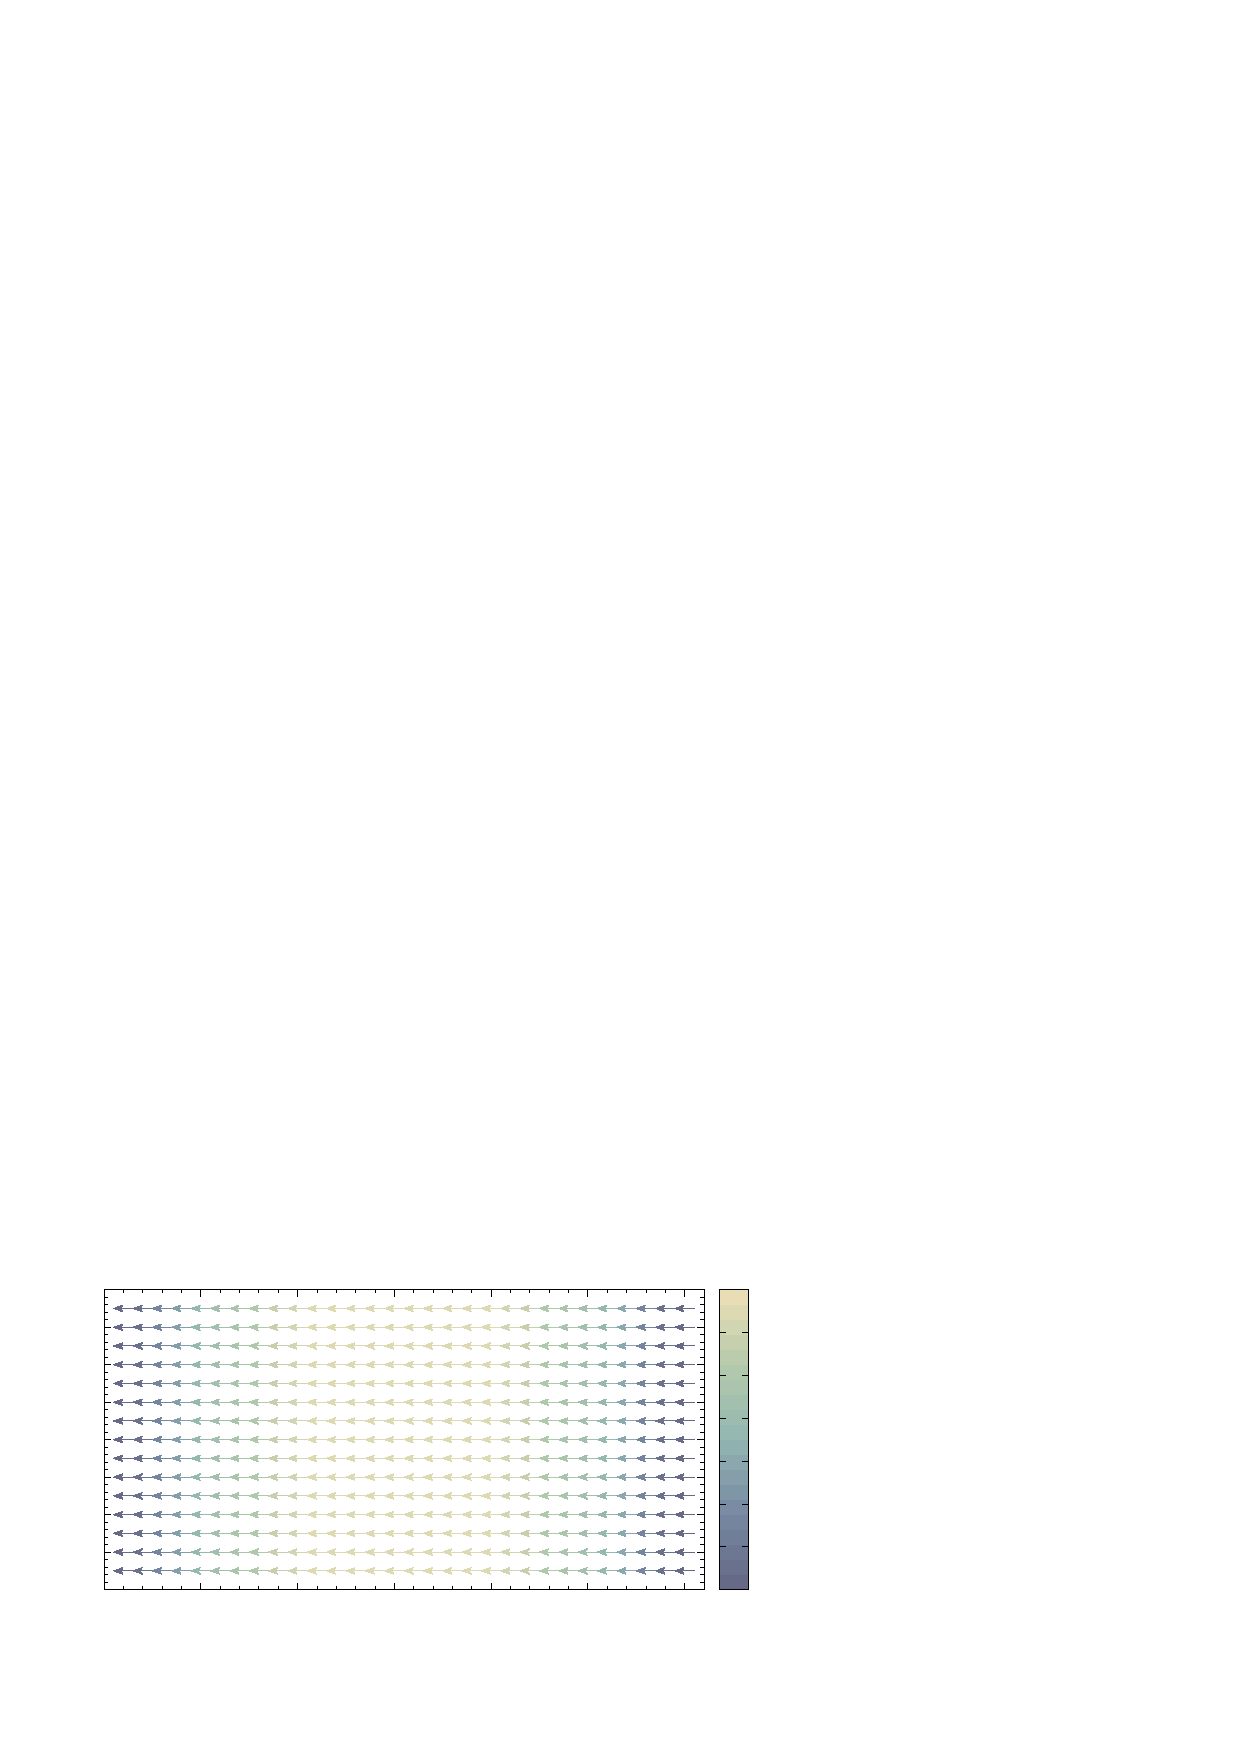
\includegraphics[width={288.00bp},height={188.60bp}]{Plots/SC10AM10/HeatMap/VertHorizBC/plot}}%
    \gplfronttext
  \end{picture}%
\endgroup


  \caption{The expectation value of the c operators taking part into the gap as $\Delta_i = U_i\langle c_{i\uparrow}c_{i\downarrow}\rangle$. The  
  vertical periodic boundary condition makes each site on the same $x$-coordinate having the same value.
    We can then make an average on each of these collumns and polt the result.}
\end{figure}
The superconducting gap lays arround $0.01\cdot U$ and $0.16\cdot U$ \rem{eV?} for the range of selected chemical potentials. Further we observe a 
clear symmetry in the Cooper pairs distribution arround the level $\mu =0$. The overlapp of the Fermi surface with the s-wave seams
to be the same for $\pm\mu$ (see Fig. \ref{fig:Brillouin}). In fact if the accessible states are also found where the superconducting gap 
is defined, we expect the electrons to be more likely to bind into Cooper pairs.\\   
Further we observe some oscillations on the left and right sides. On these locations the sites have only three
neigbhours, there are open boundaries, the rest is vaccum. One can see this lack of neigbhours as impurties in the system. 
These oscillations may be caused by Andrev bound states \cite{Bobkov_2024}, that may form because the quasiparticles are reflected at the boundary.
These can interfer with the Cooper pairs and cause the oscillations in the spacial representation of the energy gap. This is the case for the four to 
five first sites from the sides.\\
\begin{figure}[H]
  \centering
  \includegraphics[width=0.5\textwidth]{Ressources/GapBrillouin.png}
  \caption{The first Brilloun zone with the Fermi surface for $\mu$ of \textcolor{Brillou1}{$\bm{-3.8}$}, \textcolor{Brillou2}{$\bm{0}$},
  \textcolor{Brillou3}{$\bm{1.4}$} and \textcolor{Brillou4}{$\bm{3.8}$}. The BCS gap is represented by the black circle. It size is given such that 
  we can see that at a $\mu>0$ the states that can be found in the gap are less present until they vanish for a high $\mu$. For low $\mu$ there is
  not much states accessible to fill the gap as well. Figure made with Desmos.}
  \label{fig:Brillouin}
\end{figure}
In the simulation the size of the gap seams to be such, that the Fermi surface 
covers the same area of the gap representation in reciprocal space for $\pm\mu$.
A maximum arround $\mu=0$ is expected as the Fermi surface is the largest there.   

From this we can complexify the system by adding a different material on the right side of the superconductor. 
The most simple one is a normal metal (N) that has a hopping $t$ of $1$ in every direction.
Then we can repalce it with an alternating hopping $t+m$ depending on a $\uparrow\uparrow$ interaction
and a $t-m$ depending on a $\downarrow\downarrow$ interaction. This is a ferromagnetic material (FM).
Making the sign of $m$ alternating if we have an interaction along the $x$ or the $y$ axis describes an altermagnet (AM).
Here we set $m=0.5$ and study different results for the chemical potential $\mu<0$ and compare the AM
with the others. $\ast$ represent a placeholder for the material a curve describes.\\
\begin{figure}[H]
  \centering
  % GNUPLOT: LaTeX picture with Postscript
\begingroup
  % Encoding inside the plot.  In the header of your document, this encoding
  % should to defined, e.g., by using
  % \usepackage[cp1252,<other encodings>]{inputenc}
  \inputencoding{cp1252}%
  \makeatletter
  \providecommand\color[2][]{%
    \GenericError{(gnuplot) \space\space\space\@spaces}{%
      Package color not loaded in conjunction with
      terminal option `colourtext'%
    }{See the gnuplot documentation for explanation.%
    }{Either use 'blacktext' in gnuplot or load the package
      color.sty in LaTeX.}%
    \renewcommand\color[2][]{}%
  }%
  \providecommand\includegraphics[2][]{%
    \GenericError{(gnuplot) \space\space\space\@spaces}{%
      Package graphicx or graphics not loaded%
    }{See the gnuplot documentation for explanation.%
    }{The gnuplot epslatex terminal needs graphicx.sty or graphics.sty.}%
    \renewcommand\includegraphics[2][]{}%
  }%
  \providecommand\rotatebox[2]{#2}%
  \@ifundefined{ifGPcolor}{%
    \newif\ifGPcolor
    \GPcolortrue
  }{}%
  \@ifundefined{ifGPblacktext}{%
    \newif\ifGPblacktext
    \GPblacktextfalse
  }{}%
  % define a \g@addto@macro without @ in the name:
  \let\gplgaddtomacro\g@addto@macro
  % define empty templates for all commands taking text:
  \gdef\gplbacktext{}%
  \gdef\gplfronttext{}%
  \makeatother
  \ifGPblacktext
    % no textcolor at all
    \def\colorrgb#1{}%
    \def\colorgray#1{}%
  \else
    % gray or color?
    \ifGPcolor
      \def\colorrgb#1{\color[rgb]{#1}}%
      \def\colorgray#1{\color[gray]{#1}}%
      \expandafter\def\csname LTw\endcsname{\color{white}}%
      \expandafter\def\csname LTb\endcsname{\color{black}}%
      \expandafter\def\csname LTa\endcsname{\color{black}}%
      \expandafter\def\csname LT0\endcsname{\color[rgb]{1,0,0}}%
      \expandafter\def\csname LT1\endcsname{\color[rgb]{0,1,0}}%
      \expandafter\def\csname LT2\endcsname{\color[rgb]{0,0,1}}%
      \expandafter\def\csname LT3\endcsname{\color[rgb]{1,0,1}}%
      \expandafter\def\csname LT4\endcsname{\color[rgb]{0,1,1}}%
      \expandafter\def\csname LT5\endcsname{\color[rgb]{1,1,0}}%
      \expandafter\def\csname LT6\endcsname{\color[rgb]{0,0,0}}%
      \expandafter\def\csname LT7\endcsname{\color[rgb]{1,0.3,0}}%
      \expandafter\def\csname LT8\endcsname{\color[rgb]{0.5,0.5,0.5}}%
    \else
      % gray
      \def\colorrgb#1{\color{black}}%
      \def\colorgray#1{\color[gray]{#1}}%
      \expandafter\def\csname LTw\endcsname{\color{white}}%
      \expandafter\def\csname LTb\endcsname{\color{black}}%
      \expandafter\def\csname LTa\endcsname{\color{black}}%
      \expandafter\def\csname LT0\endcsname{\color{black}}%
      \expandafter\def\csname LT1\endcsname{\color{black}}%
      \expandafter\def\csname LT2\endcsname{\color{black}}%
      \expandafter\def\csname LT3\endcsname{\color{black}}%
      \expandafter\def\csname LT4\endcsname{\color{black}}%
      \expandafter\def\csname LT5\endcsname{\color{black}}%
      \expandafter\def\csname LT6\endcsname{\color{black}}%
      \expandafter\def\csname LT7\endcsname{\color{black}}%
      \expandafter\def\csname LT8\endcsname{\color{black}}%
    \fi
  \fi
    \setlength{\unitlength}{0.0500bp}%
    \ifx\gptboxheight\undefined%
      \newlength{\gptboxheight}%
      \newlength{\gptboxwidth}%
      \newsavebox{\gptboxtext}%
    \fi%
    \setlength{\fboxrule}{0.5pt}%
    \setlength{\fboxsep}{1pt}%
    \definecolor{tbcol}{rgb}{1,1,1}%
\begin{picture}(5760.00,3772.00)%
    \gplgaddtomacro\gplbacktext{%
      \csname LTb\endcsname%%
      \put(1807,3313){\makebox(0,0){\strut{}SC}}%
      \put(3953,3313){\makebox(0,0){\strut{}AM}}%
    }%
    \gplgaddtomacro\gplfronttext{%
      \csname LTb\endcsname%%
      \put(1073,742){\makebox(0,0){\scriptsize 2}}%
      \put(1525,742){\makebox(0,0){\scriptsize 4}}%
      \put(1977,742){\makebox(0,0){\scriptsize 6}}%
      \put(2429,742){\makebox(0,0){\scriptsize 8}}%
      \put(2880,742){\makebox(0,0){\scriptsize 10}}%
      \put(3331,742){\makebox(0,0){\scriptsize 12}}%
      \put(3783,742){\makebox(0,0){\scriptsize 14}}%
      \put(4235,742){\makebox(0,0){\scriptsize 16}}%
      \put(4687,742){\makebox(0,0){\scriptsize 18}}%
      \put(2880,478){\makebox(0,0){\small\textbf{Lattice site $i_x$ in $\bm{e}_x$}}}%
      \put(480,1006){\makebox(0,0){\scriptsize 2}}%
      \put(480,1254){\makebox(0,0){\scriptsize 4}}%
      \put(480,1501){\makebox(0,0){\scriptsize 6}}%
      \put(480,1749){\makebox(0,0){\scriptsize 8}}%
      \put(480,1996){\makebox(0,0){\scriptsize 10}}%
      \put(480,2243){\makebox(0,0){\scriptsize 12}}%
      \put(480,2491){\makebox(0,0){\scriptsize 14}}%
      \put(480,2738){\makebox(0,0){\scriptsize 16}}%
      \put(480,2986){\makebox(0,0){\scriptsize 18}}%
      \put(150,1996){\rotatebox{-270.00}{\makebox(0,0){\small\textbf{Lattice site $i_y$ in $\bm{e}_y$}}}}%
      \put(5743,820){\makebox(0,0){\tiny \(0\)}}%
      \put(5743,1212){\makebox(0,0){\tiny \(1e{-06}\)}}%
      \put(5743,1604){\makebox(0,0){\tiny \(2e{-06}\)}}%
      \put(5743,1996){\makebox(0,0){\tiny \(3e{-06}\)}}%
      \put(5743,2388){\makebox(0,0){\tiny \(4e{-06}\)}}%
      \put(5743,2780){\makebox(0,0){\tiny \(5e{-06}\)}}%
      \put(5743,3171){\makebox(0,0){\tiny \(6e{-06}\)}}%
    }%
    \gplbacktext
    \put(0,0){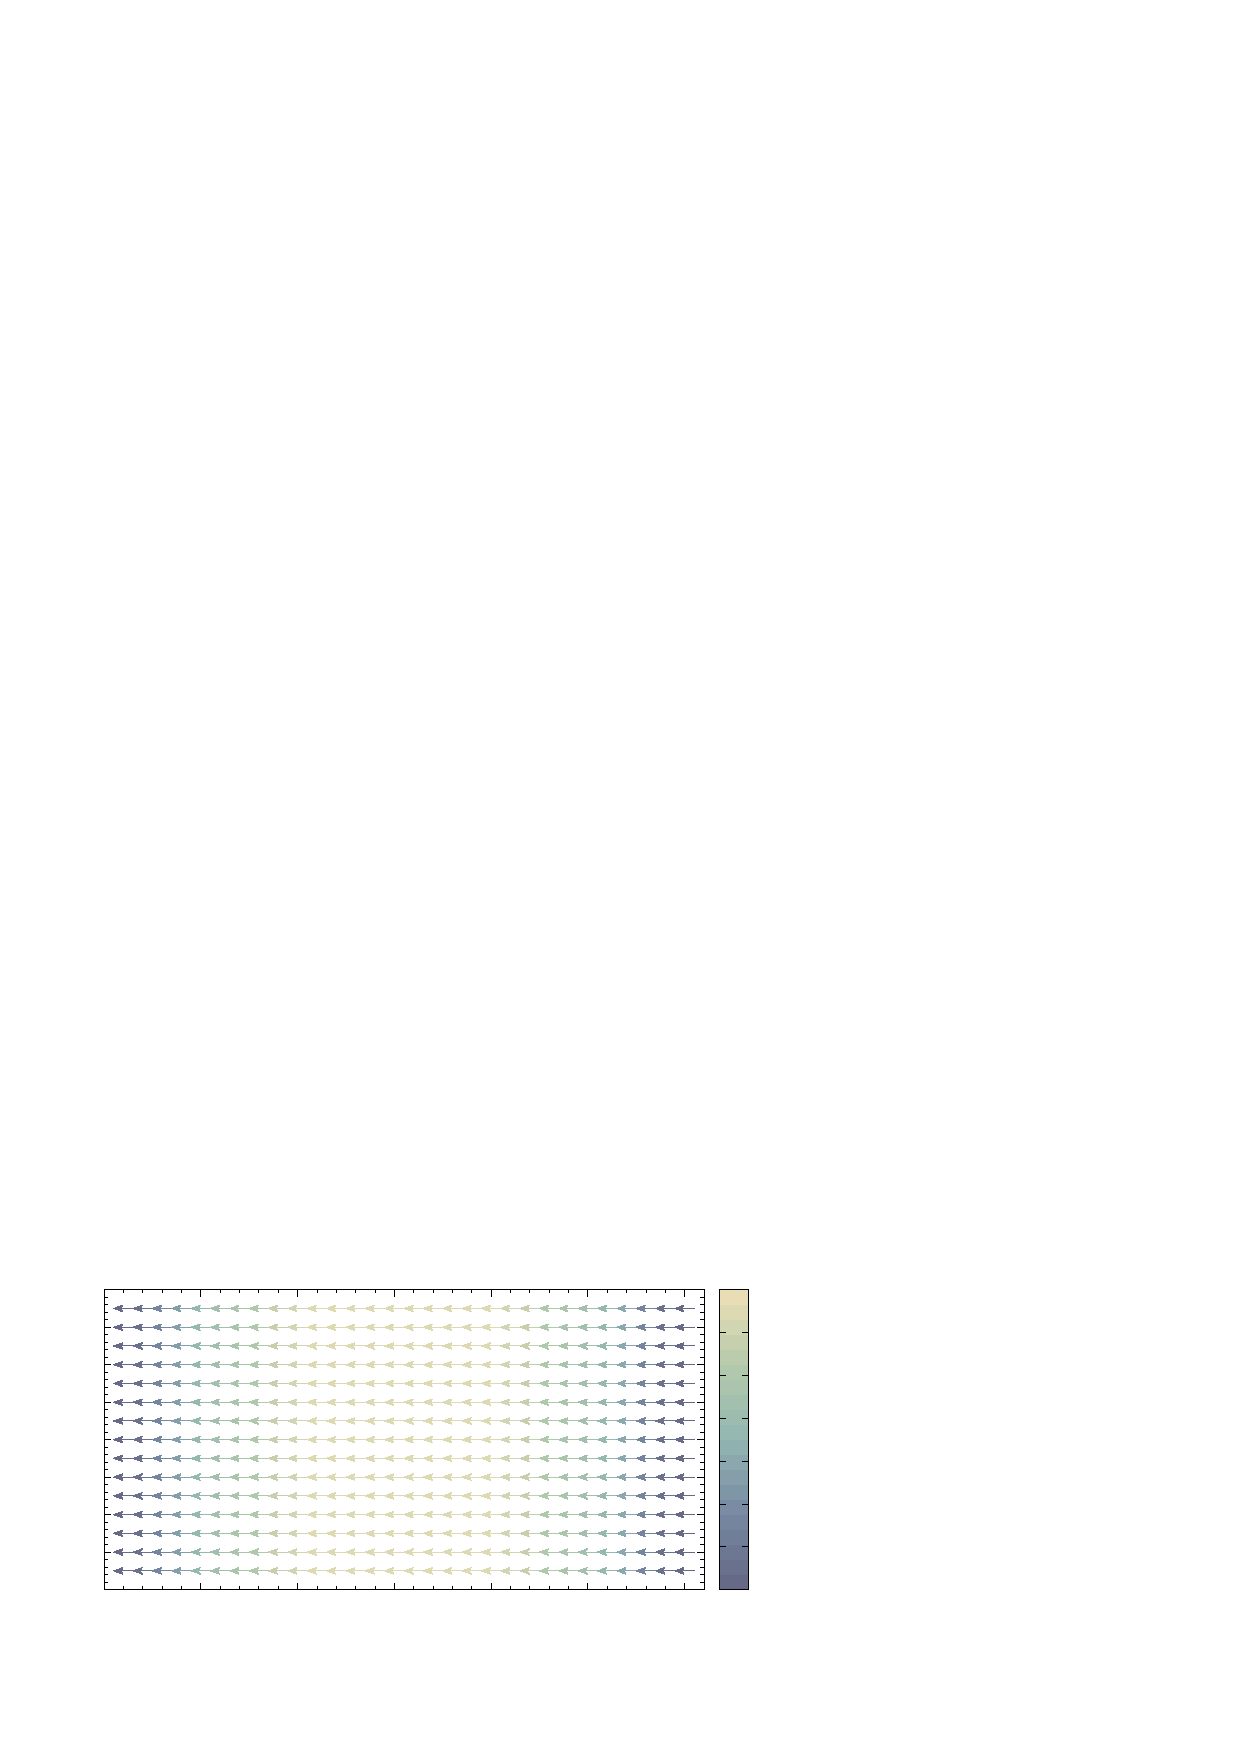
\includegraphics[width={288.00bp},height={188.60bp}]{Plots/SC10AM10/HeatMap/VertHorizBC/plot}}%
    \gplfronttext
  \end{picture}%
\endgroup


  \caption{Evolution of the gap in the $x$ direction for a junction of SC-N SC-FM and SC-AM at $\mu=-0.5$.}
\end{figure}\begin{figure}[H]
  \centering
  % GNUPLOT: LaTeX picture with Postscript
\begingroup
  % Encoding inside the plot.  In the header of your document, this encoding
  % should to defined, e.g., by using
  % \usepackage[cp1252,<other encodings>]{inputenc}
  \inputencoding{cp1252}%
  \makeatletter
  \providecommand\color[2][]{%
    \GenericError{(gnuplot) \space\space\space\@spaces}{%
      Package color not loaded in conjunction with
      terminal option `colourtext'%
    }{See the gnuplot documentation for explanation.%
    }{Either use 'blacktext' in gnuplot or load the package
      color.sty in LaTeX.}%
    \renewcommand\color[2][]{}%
  }%
  \providecommand\includegraphics[2][]{%
    \GenericError{(gnuplot) \space\space\space\@spaces}{%
      Package graphicx or graphics not loaded%
    }{See the gnuplot documentation for explanation.%
    }{The gnuplot epslatex terminal needs graphicx.sty or graphics.sty.}%
    \renewcommand\includegraphics[2][]{}%
  }%
  \providecommand\rotatebox[2]{#2}%
  \@ifundefined{ifGPcolor}{%
    \newif\ifGPcolor
    \GPcolortrue
  }{}%
  \@ifundefined{ifGPblacktext}{%
    \newif\ifGPblacktext
    \GPblacktextfalse
  }{}%
  % define a \g@addto@macro without @ in the name:
  \let\gplgaddtomacro\g@addto@macro
  % define empty templates for all commands taking text:
  \gdef\gplbacktext{}%
  \gdef\gplfronttext{}%
  \makeatother
  \ifGPblacktext
    % no textcolor at all
    \def\colorrgb#1{}%
    \def\colorgray#1{}%
  \else
    % gray or color?
    \ifGPcolor
      \def\colorrgb#1{\color[rgb]{#1}}%
      \def\colorgray#1{\color[gray]{#1}}%
      \expandafter\def\csname LTw\endcsname{\color{white}}%
      \expandafter\def\csname LTb\endcsname{\color{black}}%
      \expandafter\def\csname LTa\endcsname{\color{black}}%
      \expandafter\def\csname LT0\endcsname{\color[rgb]{1,0,0}}%
      \expandafter\def\csname LT1\endcsname{\color[rgb]{0,1,0}}%
      \expandafter\def\csname LT2\endcsname{\color[rgb]{0,0,1}}%
      \expandafter\def\csname LT3\endcsname{\color[rgb]{1,0,1}}%
      \expandafter\def\csname LT4\endcsname{\color[rgb]{0,1,1}}%
      \expandafter\def\csname LT5\endcsname{\color[rgb]{1,1,0}}%
      \expandafter\def\csname LT6\endcsname{\color[rgb]{0,0,0}}%
      \expandafter\def\csname LT7\endcsname{\color[rgb]{1,0.3,0}}%
      \expandafter\def\csname LT8\endcsname{\color[rgb]{0.5,0.5,0.5}}%
    \else
      % gray
      \def\colorrgb#1{\color{black}}%
      \def\colorgray#1{\color[gray]{#1}}%
      \expandafter\def\csname LTw\endcsname{\color{white}}%
      \expandafter\def\csname LTb\endcsname{\color{black}}%
      \expandafter\def\csname LTa\endcsname{\color{black}}%
      \expandafter\def\csname LT0\endcsname{\color{black}}%
      \expandafter\def\csname LT1\endcsname{\color{black}}%
      \expandafter\def\csname LT2\endcsname{\color{black}}%
      \expandafter\def\csname LT3\endcsname{\color{black}}%
      \expandafter\def\csname LT4\endcsname{\color{black}}%
      \expandafter\def\csname LT5\endcsname{\color{black}}%
      \expandafter\def\csname LT6\endcsname{\color{black}}%
      \expandafter\def\csname LT7\endcsname{\color{black}}%
      \expandafter\def\csname LT8\endcsname{\color{black}}%
    \fi
  \fi
    \setlength{\unitlength}{0.0500bp}%
    \ifx\gptboxheight\undefined%
      \newlength{\gptboxheight}%
      \newlength{\gptboxwidth}%
      \newsavebox{\gptboxtext}%
    \fi%
    \setlength{\fboxrule}{0.5pt}%
    \setlength{\fboxsep}{1pt}%
    \definecolor{tbcol}{rgb}{1,1,1}%
\begin{picture}(5760.00,3772.00)%
    \gplgaddtomacro\gplbacktext{%
      \csname LTb\endcsname%%
      \put(1807,3313){\makebox(0,0){\strut{}SC}}%
      \put(3953,3313){\makebox(0,0){\strut{}AM}}%
    }%
    \gplgaddtomacro\gplfronttext{%
      \csname LTb\endcsname%%
      \put(1073,742){\makebox(0,0){\scriptsize 2}}%
      \put(1525,742){\makebox(0,0){\scriptsize 4}}%
      \put(1977,742){\makebox(0,0){\scriptsize 6}}%
      \put(2429,742){\makebox(0,0){\scriptsize 8}}%
      \put(2880,742){\makebox(0,0){\scriptsize 10}}%
      \put(3331,742){\makebox(0,0){\scriptsize 12}}%
      \put(3783,742){\makebox(0,0){\scriptsize 14}}%
      \put(4235,742){\makebox(0,0){\scriptsize 16}}%
      \put(4687,742){\makebox(0,0){\scriptsize 18}}%
      \put(2880,478){\makebox(0,0){\small\textbf{Lattice site $i_x$ in $\bm{e}_x$}}}%
      \put(480,1006){\makebox(0,0){\scriptsize 2}}%
      \put(480,1254){\makebox(0,0){\scriptsize 4}}%
      \put(480,1501){\makebox(0,0){\scriptsize 6}}%
      \put(480,1749){\makebox(0,0){\scriptsize 8}}%
      \put(480,1996){\makebox(0,0){\scriptsize 10}}%
      \put(480,2243){\makebox(0,0){\scriptsize 12}}%
      \put(480,2491){\makebox(0,0){\scriptsize 14}}%
      \put(480,2738){\makebox(0,0){\scriptsize 16}}%
      \put(480,2986){\makebox(0,0){\scriptsize 18}}%
      \put(150,1996){\rotatebox{-270.00}{\makebox(0,0){\small\textbf{Lattice site $i_y$ in $\bm{e}_y$}}}}%
      \put(5743,820){\makebox(0,0){\tiny \(0\)}}%
      \put(5743,1212){\makebox(0,0){\tiny \(1e{-06}\)}}%
      \put(5743,1604){\makebox(0,0){\tiny \(2e{-06}\)}}%
      \put(5743,1996){\makebox(0,0){\tiny \(3e{-06}\)}}%
      \put(5743,2388){\makebox(0,0){\tiny \(4e{-06}\)}}%
      \put(5743,2780){\makebox(0,0){\tiny \(5e{-06}\)}}%
      \put(5743,3171){\makebox(0,0){\tiny \(6e{-06}\)}}%
    }%
    \gplbacktext
    \put(0,0){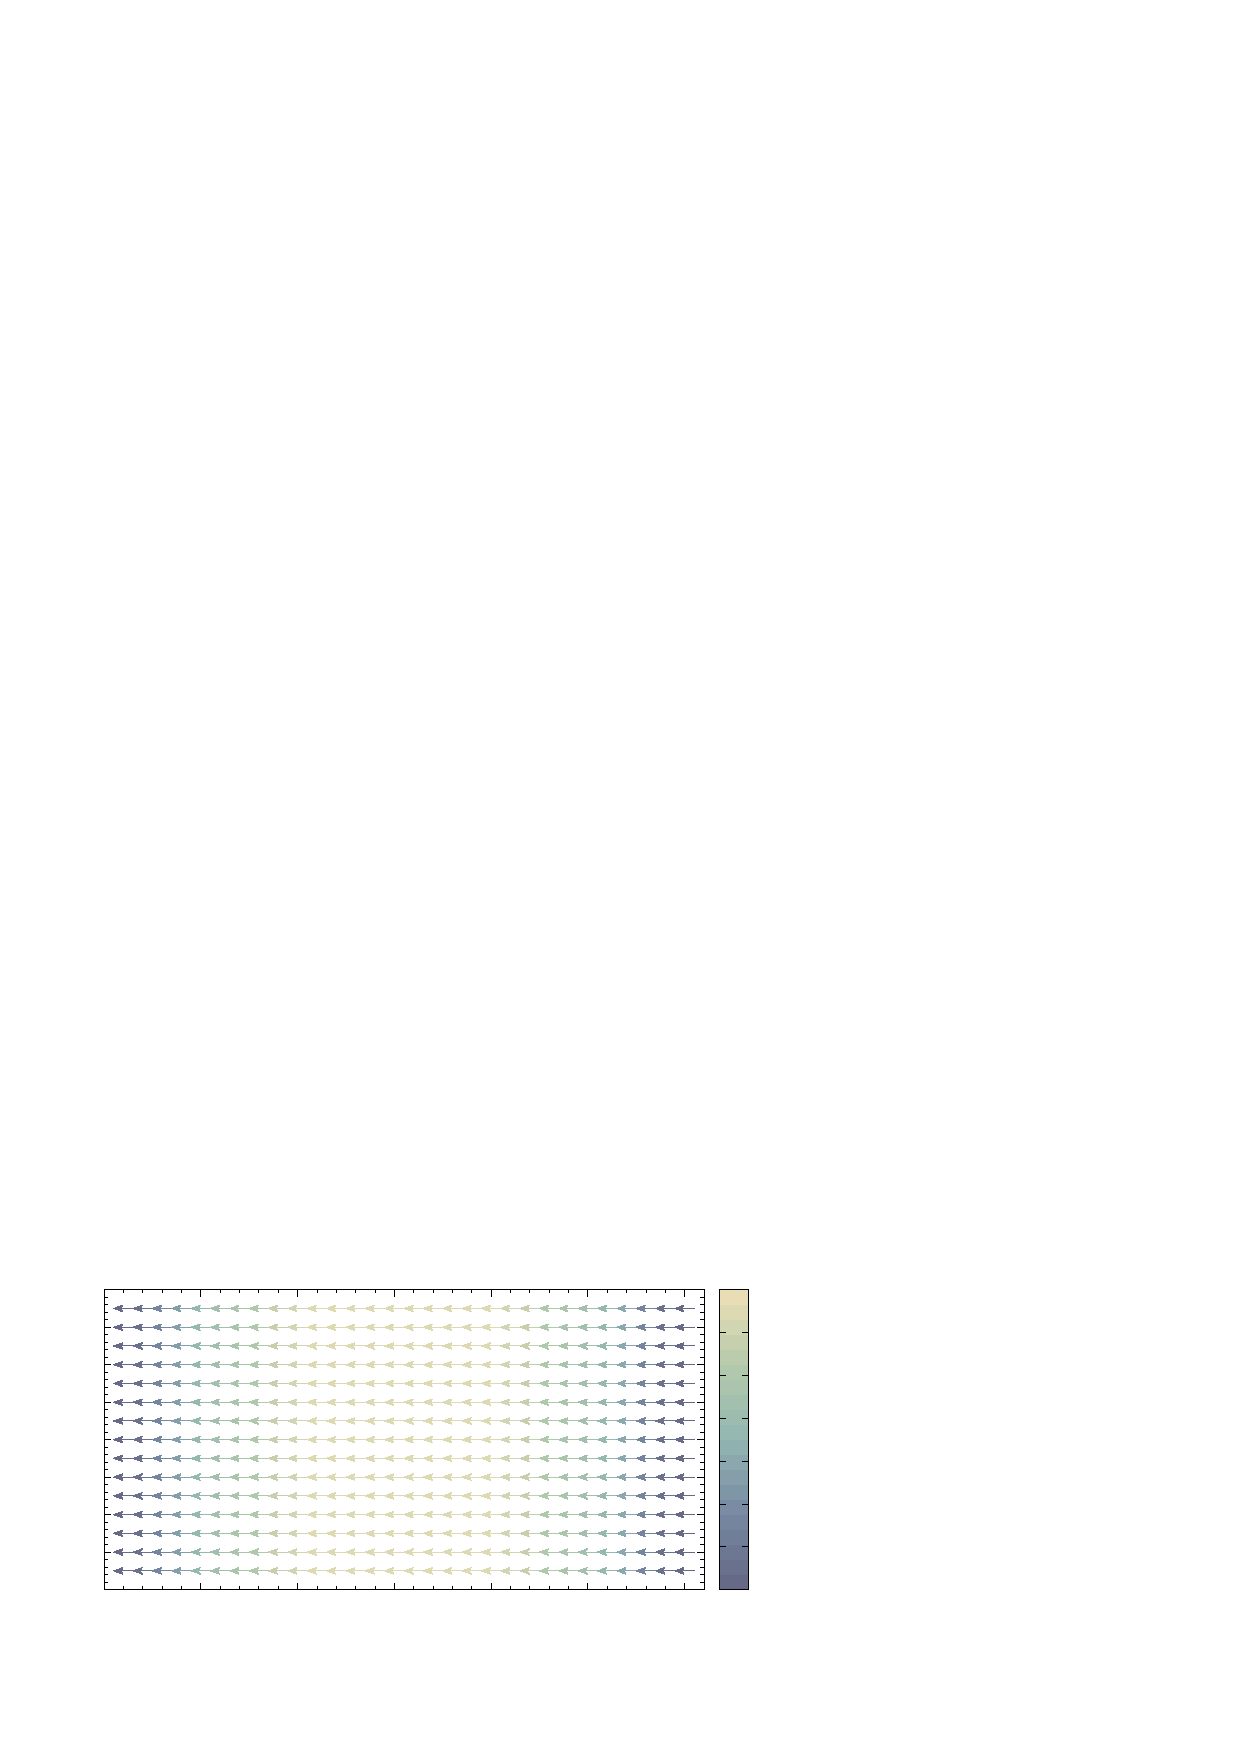
\includegraphics[width={288.00bp},height={188.60bp}]{Plots/SC10AM10/HeatMap/VertHorizBC/plot}}%
    \gplfronttext
  \end{picture}%
\endgroup


  \caption{Evolution of the gap in the $x$ direction for a junction of SC-N SC-FM and SC-AM at $\mu=-1.5$.}
\end{figure}
\begin{figure}[H]
  \centering
  % GNUPLOT: LaTeX picture with Postscript
\begingroup
  % Encoding inside the plot.  In the header of your document, this encoding
  % should to defined, e.g., by using
  % \usepackage[cp1252,<other encodings>]{inputenc}
  \inputencoding{cp1252}%
  \makeatletter
  \providecommand\color[2][]{%
    \GenericError{(gnuplot) \space\space\space\@spaces}{%
      Package color not loaded in conjunction with
      terminal option `colourtext'%
    }{See the gnuplot documentation for explanation.%
    }{Either use 'blacktext' in gnuplot or load the package
      color.sty in LaTeX.}%
    \renewcommand\color[2][]{}%
  }%
  \providecommand\includegraphics[2][]{%
    \GenericError{(gnuplot) \space\space\space\@spaces}{%
      Package graphicx or graphics not loaded%
    }{See the gnuplot documentation for explanation.%
    }{The gnuplot epslatex terminal needs graphicx.sty or graphics.sty.}%
    \renewcommand\includegraphics[2][]{}%
  }%
  \providecommand\rotatebox[2]{#2}%
  \@ifundefined{ifGPcolor}{%
    \newif\ifGPcolor
    \GPcolortrue
  }{}%
  \@ifundefined{ifGPblacktext}{%
    \newif\ifGPblacktext
    \GPblacktextfalse
  }{}%
  % define a \g@addto@macro without @ in the name:
  \let\gplgaddtomacro\g@addto@macro
  % define empty templates for all commands taking text:
  \gdef\gplbacktext{}%
  \gdef\gplfronttext{}%
  \makeatother
  \ifGPblacktext
    % no textcolor at all
    \def\colorrgb#1{}%
    \def\colorgray#1{}%
  \else
    % gray or color?
    \ifGPcolor
      \def\colorrgb#1{\color[rgb]{#1}}%
      \def\colorgray#1{\color[gray]{#1}}%
      \expandafter\def\csname LTw\endcsname{\color{white}}%
      \expandafter\def\csname LTb\endcsname{\color{black}}%
      \expandafter\def\csname LTa\endcsname{\color{black}}%
      \expandafter\def\csname LT0\endcsname{\color[rgb]{1,0,0}}%
      \expandafter\def\csname LT1\endcsname{\color[rgb]{0,1,0}}%
      \expandafter\def\csname LT2\endcsname{\color[rgb]{0,0,1}}%
      \expandafter\def\csname LT3\endcsname{\color[rgb]{1,0,1}}%
      \expandafter\def\csname LT4\endcsname{\color[rgb]{0,1,1}}%
      \expandafter\def\csname LT5\endcsname{\color[rgb]{1,1,0}}%
      \expandafter\def\csname LT6\endcsname{\color[rgb]{0,0,0}}%
      \expandafter\def\csname LT7\endcsname{\color[rgb]{1,0.3,0}}%
      \expandafter\def\csname LT8\endcsname{\color[rgb]{0.5,0.5,0.5}}%
    \else
      % gray
      \def\colorrgb#1{\color{black}}%
      \def\colorgray#1{\color[gray]{#1}}%
      \expandafter\def\csname LTw\endcsname{\color{white}}%
      \expandafter\def\csname LTb\endcsname{\color{black}}%
      \expandafter\def\csname LTa\endcsname{\color{black}}%
      \expandafter\def\csname LT0\endcsname{\color{black}}%
      \expandafter\def\csname LT1\endcsname{\color{black}}%
      \expandafter\def\csname LT2\endcsname{\color{black}}%
      \expandafter\def\csname LT3\endcsname{\color{black}}%
      \expandafter\def\csname LT4\endcsname{\color{black}}%
      \expandafter\def\csname LT5\endcsname{\color{black}}%
      \expandafter\def\csname LT6\endcsname{\color{black}}%
      \expandafter\def\csname LT7\endcsname{\color{black}}%
      \expandafter\def\csname LT8\endcsname{\color{black}}%
    \fi
  \fi
    \setlength{\unitlength}{0.0500bp}%
    \ifx\gptboxheight\undefined%
      \newlength{\gptboxheight}%
      \newlength{\gptboxwidth}%
      \newsavebox{\gptboxtext}%
    \fi%
    \setlength{\fboxrule}{0.5pt}%
    \setlength{\fboxsep}{1pt}%
    \definecolor{tbcol}{rgb}{1,1,1}%
\begin{picture}(5760.00,3772.00)%
    \gplgaddtomacro\gplbacktext{%
      \csname LTb\endcsname%%
      \put(1807,3313){\makebox(0,0){\strut{}SC}}%
      \put(3953,3313){\makebox(0,0){\strut{}AM}}%
    }%
    \gplgaddtomacro\gplfronttext{%
      \csname LTb\endcsname%%
      \put(1073,742){\makebox(0,0){\scriptsize 2}}%
      \put(1525,742){\makebox(0,0){\scriptsize 4}}%
      \put(1977,742){\makebox(0,0){\scriptsize 6}}%
      \put(2429,742){\makebox(0,0){\scriptsize 8}}%
      \put(2880,742){\makebox(0,0){\scriptsize 10}}%
      \put(3331,742){\makebox(0,0){\scriptsize 12}}%
      \put(3783,742){\makebox(0,0){\scriptsize 14}}%
      \put(4235,742){\makebox(0,0){\scriptsize 16}}%
      \put(4687,742){\makebox(0,0){\scriptsize 18}}%
      \put(2880,478){\makebox(0,0){\small\textbf{Lattice site $i_x$ in $\bm{e}_x$}}}%
      \put(480,1006){\makebox(0,0){\scriptsize 2}}%
      \put(480,1254){\makebox(0,0){\scriptsize 4}}%
      \put(480,1501){\makebox(0,0){\scriptsize 6}}%
      \put(480,1749){\makebox(0,0){\scriptsize 8}}%
      \put(480,1996){\makebox(0,0){\scriptsize 10}}%
      \put(480,2243){\makebox(0,0){\scriptsize 12}}%
      \put(480,2491){\makebox(0,0){\scriptsize 14}}%
      \put(480,2738){\makebox(0,0){\scriptsize 16}}%
      \put(480,2986){\makebox(0,0){\scriptsize 18}}%
      \put(150,1996){\rotatebox{-270.00}{\makebox(0,0){\small\textbf{Lattice site $i_y$ in $\bm{e}_y$}}}}%
      \put(5743,820){\makebox(0,0){\tiny \(0\)}}%
      \put(5743,1212){\makebox(0,0){\tiny \(1e{-06}\)}}%
      \put(5743,1604){\makebox(0,0){\tiny \(2e{-06}\)}}%
      \put(5743,1996){\makebox(0,0){\tiny \(3e{-06}\)}}%
      \put(5743,2388){\makebox(0,0){\tiny \(4e{-06}\)}}%
      \put(5743,2780){\makebox(0,0){\tiny \(5e{-06}\)}}%
      \put(5743,3171){\makebox(0,0){\tiny \(6e{-06}\)}}%
    }%
    \gplbacktext
    \put(0,0){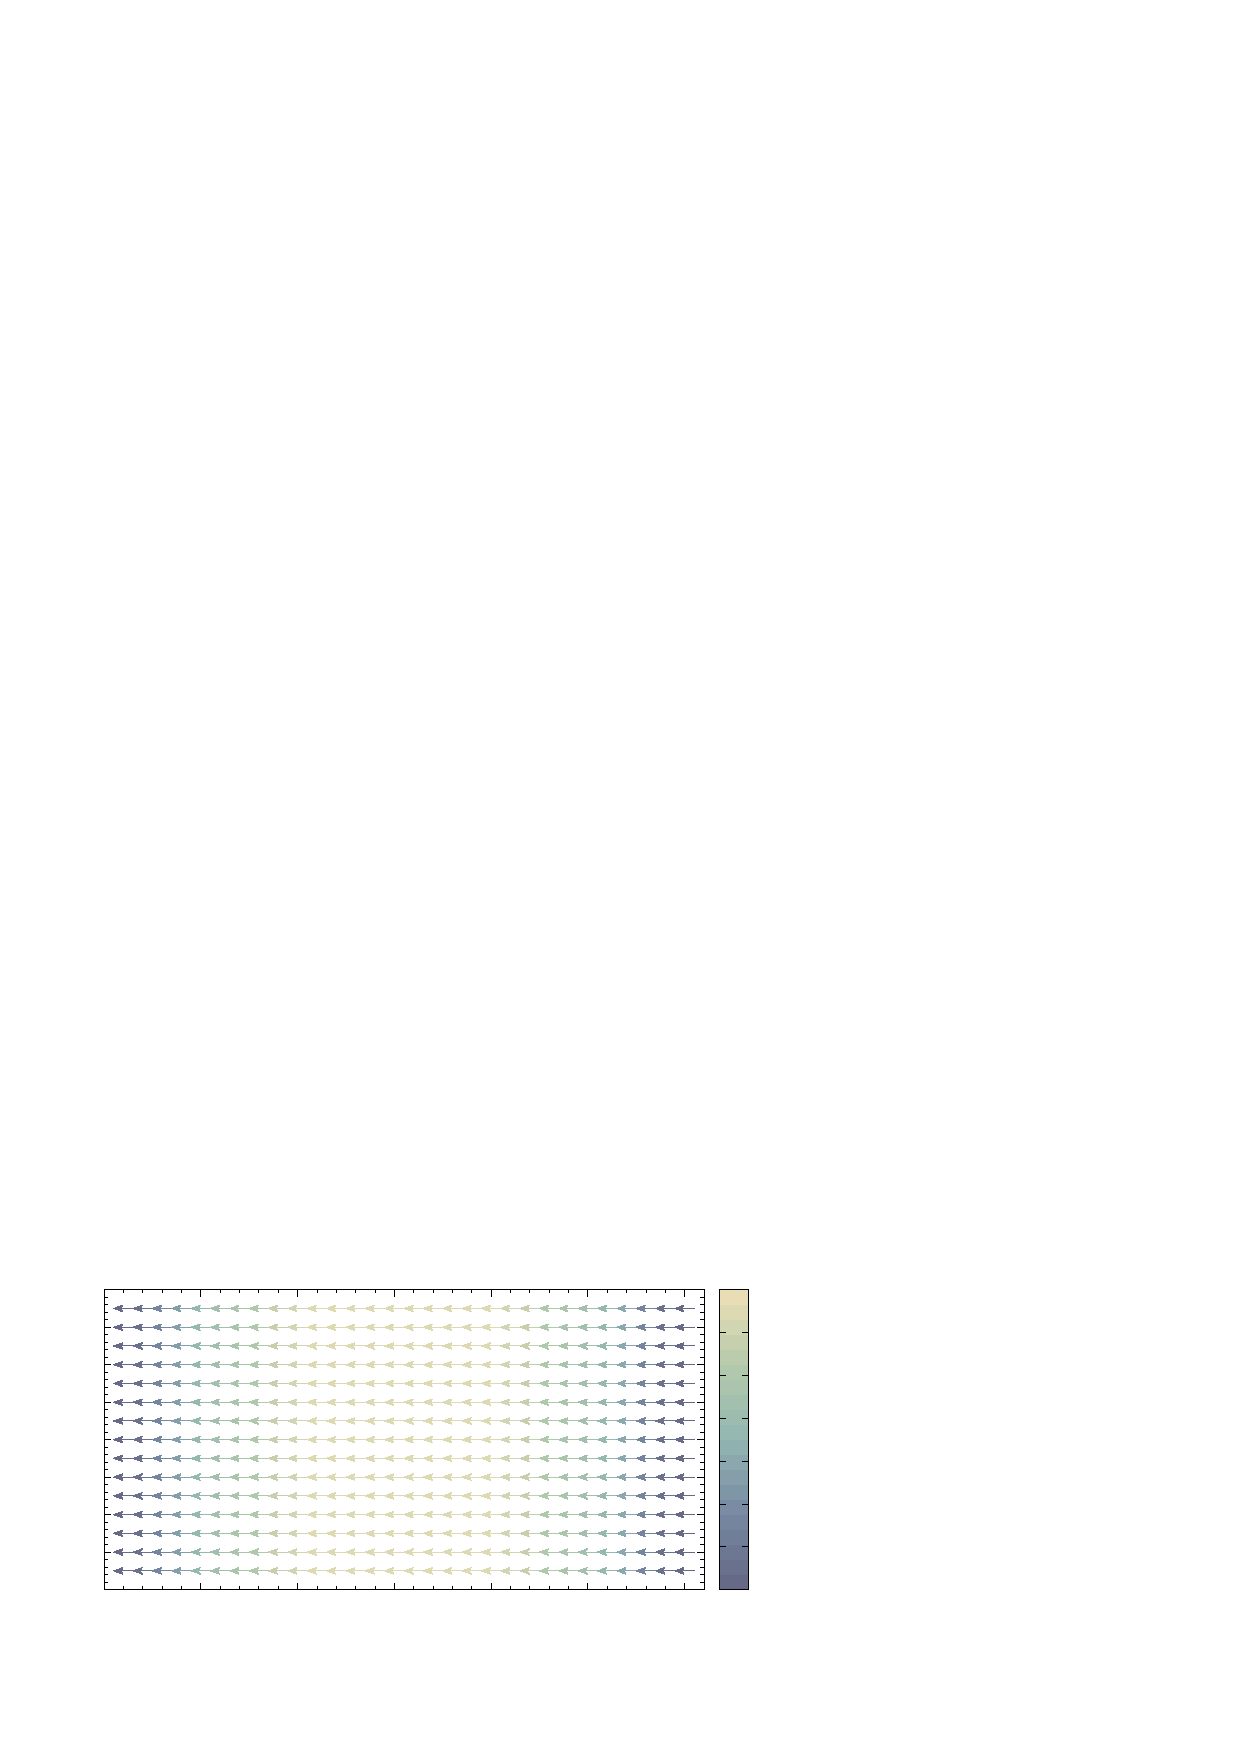
\includegraphics[width={288.00bp},height={188.60bp}]{Plots/SC10AM10/HeatMap/VertHorizBC/plot}}%
    \gplfronttext
  \end{picture}%
\endgroup


  \caption{Evolution of the gap in the $x$ direction for a junction of SC-N SC-FM and SC-AM at $\mu=-2.5$.}
\end{figure}
We first take a look at the superconductor (SC). Inside of it the gap seams not be the same for $\mu=-0.5,-1.5$
and sattels arround $0.1\cdot U$. Most likely the increase of the Fermi surface don't seam to give an additional contribution to the gap.
The gap is however one order of magnetude smaller for $\mu=-2.5$. Here the withdraw of the Fermi surface is more relevant and the 
gap becomes smaller.\\
We have a clear decay of the gap after entering the normal metal (N). At this point 
study that were already made tend to have an exponential decay of the gap \cite{Mjos2019}. Having a logarithmic scale we would
exepect a more straight line but this is still a reasonable exponential decay. A way to approch the line would be to increase the 
resolution of the lattice, as well as simulating a more squared one. This decay makes the expectation value having an order of 
magnetude of difference from one side to the other of the N. For the smallest $\mu$ we see that the decay is weaker, the gap loosed
the half of its amplitude after crossing the N. Further we see that both the FM and the AM add some oscilations in the decay. \\

The ferromagnet seams to follow closely the normal metal for $\mu=-0.5,-1.5$. It is intersting to note a realy nice exponential
decay when having a chemical potential of $-2.5$ modulated by oscillations. We observe about the same number of oscillations and about of
the same amplitude in these three cases. In the AM the initial decay is stronger in the sites near the 
interface than in the FM. Then the decay seams to follow the FM. We observe about the same number of oscilations in the FM and the AM.
For $\mu=-0.5$ we observe a clean line in the first four sites of the AM. Than we have oscilations and the Cooper-pairs are more present
than expected regarding the initial decay. The reason might be that the first oscillation combined with the inital decay make the line
reach it's second deepest point (arround $10^{-4}$) and therfore everything looks more flat.

In the AM the oscillation amplitude seams to increased with a decreasing $|\mu|$.
We observe nearly two orders of magnetude in their amplitude for $\mu=-0.5$ compared to one order of magnetude for $\mu=-2.5$.
We tried to simualte these for a $\mu=-3.5$ but the algorithm  converge to values that are nummerically zero everywhere ($10^{-16}$).
It looks like the Fermi-surface is too small and there is a lack of electrons to build the Cooper pairs.\\
 
These oscilations are more likely due to the fact that we have a spin-dependent hopping. In fact we have the same behaviour for the AM
and the FM, but not in the N. This dynamic influences the gap and the different components of the gap interfer with eachother resulting
periodicly in espescially low values. It seams that the direction-dependence of the altermagnetic hopping causes a weaker gap and 
oscillations of bigger amplitudes. Traces of the quasiparticles reflection are still visible, espescially in the non-SC materials.\\

We now want simualte the behaviour of the s-wave superconductivity on a diagonal interface. We focus on three different values of $\mu<0$.  
The diagonal is build by rotating the interface by $45^{\circ}$ arround the center of the lattice. The upper-part, regarding the $y$-axis is the SC
and the lower one the AM. We set $m=0.5$.
\begin{figure}[H]
    \centering
    % GNUPLOT: LaTeX picture with Postscript
\begingroup
  % Encoding inside the plot.  In the header of your document, this encoding
  % should to defined, e.g., by using
  % \usepackage[cp1252,<other encodings>]{inputenc}
  \inputencoding{cp1252}%
  \makeatletter
  \providecommand\color[2][]{%
    \GenericError{(gnuplot) \space\space\space\@spaces}{%
      Package color not loaded in conjunction with
      terminal option `colourtext'%
    }{See the gnuplot documentation for explanation.%
    }{Either use 'blacktext' in gnuplot or load the package
      color.sty in LaTeX.}%
    \renewcommand\color[2][]{}%
  }%
  \providecommand\includegraphics[2][]{%
    \GenericError{(gnuplot) \space\space\space\@spaces}{%
      Package graphicx or graphics not loaded%
    }{See the gnuplot documentation for explanation.%
    }{The gnuplot epslatex terminal needs graphicx.sty or graphics.sty.}%
    \renewcommand\includegraphics[2][]{}%
  }%
  \providecommand\rotatebox[2]{#2}%
  \@ifundefined{ifGPcolor}{%
    \newif\ifGPcolor
    \GPcolortrue
  }{}%
  \@ifundefined{ifGPblacktext}{%
    \newif\ifGPblacktext
    \GPblacktextfalse
  }{}%
  % define a \g@addto@macro without @ in the name:
  \let\gplgaddtomacro\g@addto@macro
  % define empty templates for all commands taking text:
  \gdef\gplbacktext{}%
  \gdef\gplfronttext{}%
  \makeatother
  \ifGPblacktext
    % no textcolor at all
    \def\colorrgb#1{}%
    \def\colorgray#1{}%
  \else
    % gray or color?
    \ifGPcolor
      \def\colorrgb#1{\color[rgb]{#1}}%
      \def\colorgray#1{\color[gray]{#1}}%
      \expandafter\def\csname LTw\endcsname{\color{white}}%
      \expandafter\def\csname LTb\endcsname{\color{black}}%
      \expandafter\def\csname LTa\endcsname{\color{black}}%
      \expandafter\def\csname LT0\endcsname{\color[rgb]{1,0,0}}%
      \expandafter\def\csname LT1\endcsname{\color[rgb]{0,1,0}}%
      \expandafter\def\csname LT2\endcsname{\color[rgb]{0,0,1}}%
      \expandafter\def\csname LT3\endcsname{\color[rgb]{1,0,1}}%
      \expandafter\def\csname LT4\endcsname{\color[rgb]{0,1,1}}%
      \expandafter\def\csname LT5\endcsname{\color[rgb]{1,1,0}}%
      \expandafter\def\csname LT6\endcsname{\color[rgb]{0,0,0}}%
      \expandafter\def\csname LT7\endcsname{\color[rgb]{1,0.3,0}}%
      \expandafter\def\csname LT8\endcsname{\color[rgb]{0.5,0.5,0.5}}%
    \else
      % gray
      \def\colorrgb#1{\color{black}}%
      \def\colorgray#1{\color[gray]{#1}}%
      \expandafter\def\csname LTw\endcsname{\color{white}}%
      \expandafter\def\csname LTb\endcsname{\color{black}}%
      \expandafter\def\csname LTa\endcsname{\color{black}}%
      \expandafter\def\csname LT0\endcsname{\color{black}}%
      \expandafter\def\csname LT1\endcsname{\color{black}}%
      \expandafter\def\csname LT2\endcsname{\color{black}}%
      \expandafter\def\csname LT3\endcsname{\color{black}}%
      \expandafter\def\csname LT4\endcsname{\color{black}}%
      \expandafter\def\csname LT5\endcsname{\color{black}}%
      \expandafter\def\csname LT6\endcsname{\color{black}}%
      \expandafter\def\csname LT7\endcsname{\color{black}}%
      \expandafter\def\csname LT8\endcsname{\color{black}}%
    \fi
  \fi
    \setlength{\unitlength}{0.0500bp}%
    \ifx\gptboxheight\undefined%
      \newlength{\gptboxheight}%
      \newlength{\gptboxwidth}%
      \newsavebox{\gptboxtext}%
    \fi%
    \setlength{\fboxrule}{0.5pt}%
    \setlength{\fboxsep}{1pt}%
    \definecolor{tbcol}{rgb}{1,1,1}%
\begin{picture}(5760.00,3772.00)%
    \gplgaddtomacro\gplbacktext{%
      \csname LTb\endcsname%%
      \put(1807,3313){\makebox(0,0){\strut{}SC}}%
      \put(3953,3313){\makebox(0,0){\strut{}AM}}%
    }%
    \gplgaddtomacro\gplfronttext{%
      \csname LTb\endcsname%%
      \put(1073,742){\makebox(0,0){\scriptsize 2}}%
      \put(1525,742){\makebox(0,0){\scriptsize 4}}%
      \put(1977,742){\makebox(0,0){\scriptsize 6}}%
      \put(2429,742){\makebox(0,0){\scriptsize 8}}%
      \put(2880,742){\makebox(0,0){\scriptsize 10}}%
      \put(3331,742){\makebox(0,0){\scriptsize 12}}%
      \put(3783,742){\makebox(0,0){\scriptsize 14}}%
      \put(4235,742){\makebox(0,0){\scriptsize 16}}%
      \put(4687,742){\makebox(0,0){\scriptsize 18}}%
      \put(2880,478){\makebox(0,0){\small\textbf{Lattice site $i_x$ in $\bm{e}_x$}}}%
      \put(480,1006){\makebox(0,0){\scriptsize 2}}%
      \put(480,1254){\makebox(0,0){\scriptsize 4}}%
      \put(480,1501){\makebox(0,0){\scriptsize 6}}%
      \put(480,1749){\makebox(0,0){\scriptsize 8}}%
      \put(480,1996){\makebox(0,0){\scriptsize 10}}%
      \put(480,2243){\makebox(0,0){\scriptsize 12}}%
      \put(480,2491){\makebox(0,0){\scriptsize 14}}%
      \put(480,2738){\makebox(0,0){\scriptsize 16}}%
      \put(480,2986){\makebox(0,0){\scriptsize 18}}%
      \put(150,1996){\rotatebox{-270.00}{\makebox(0,0){\small\textbf{Lattice site $i_y$ in $\bm{e}_y$}}}}%
      \put(5743,820){\makebox(0,0){\tiny \(0\)}}%
      \put(5743,1212){\makebox(0,0){\tiny \(1e{-06}\)}}%
      \put(5743,1604){\makebox(0,0){\tiny \(2e{-06}\)}}%
      \put(5743,1996){\makebox(0,0){\tiny \(3e{-06}\)}}%
      \put(5743,2388){\makebox(0,0){\tiny \(4e{-06}\)}}%
      \put(5743,2780){\makebox(0,0){\tiny \(5e{-06}\)}}%
      \put(5743,3171){\makebox(0,0){\tiny \(6e{-06}\)}}%
    }%
    \gplbacktext
    \put(0,0){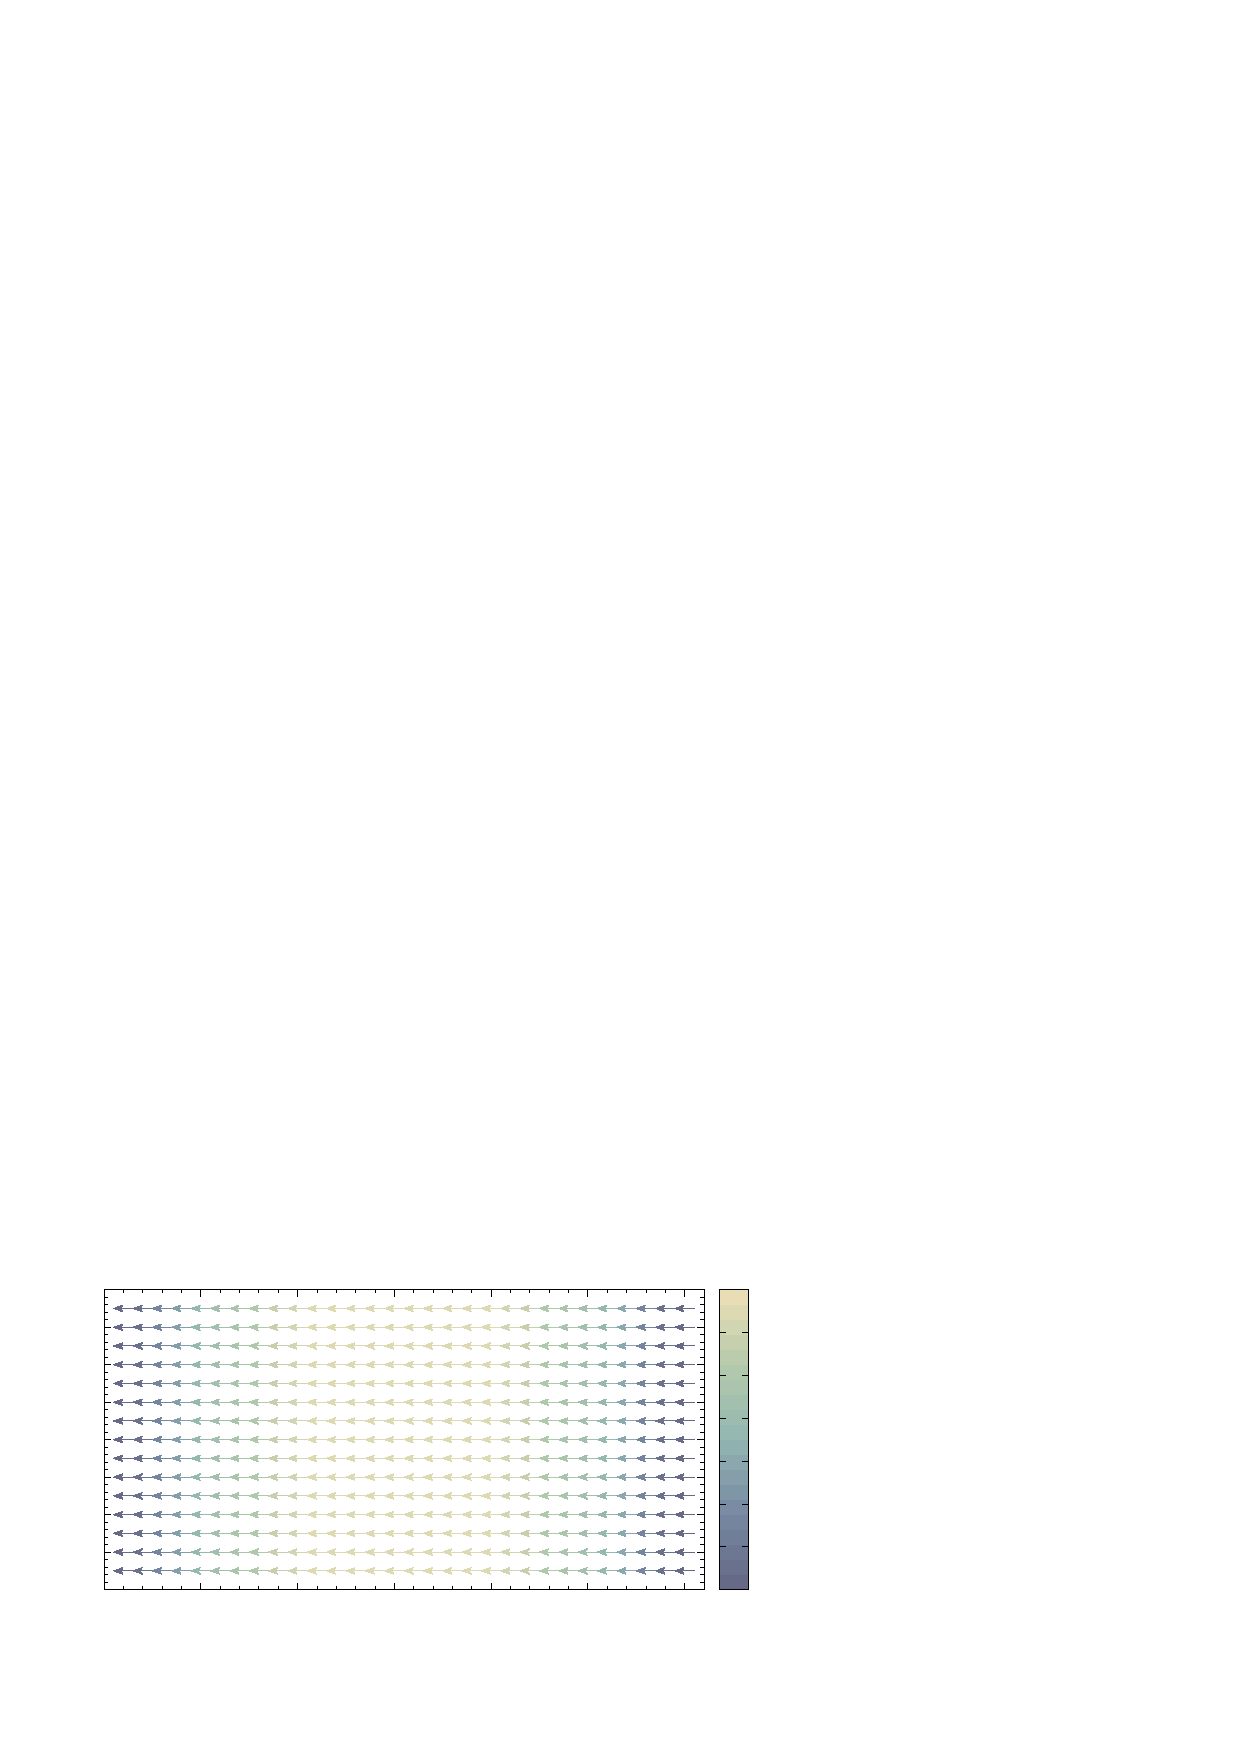
\includegraphics[width={288.00bp},height={188.60bp}]{Plots/SC10AM10/HeatMap/VertHorizBC/plot}}%
    \gplfronttext
  \end{picture}%
\endgroup


    \caption{Diagonal interface of a SC and an AM at $\mu = -2.5$.}
\end{figure}
\begin{figure}[H]
    \centering
    % GNUPLOT: LaTeX picture with Postscript
\begingroup
  % Encoding inside the plot.  In the header of your document, this encoding
  % should to defined, e.g., by using
  % \usepackage[cp1252,<other encodings>]{inputenc}
  \inputencoding{cp1252}%
  \makeatletter
  \providecommand\color[2][]{%
    \GenericError{(gnuplot) \space\space\space\@spaces}{%
      Package color not loaded in conjunction with
      terminal option `colourtext'%
    }{See the gnuplot documentation for explanation.%
    }{Either use 'blacktext' in gnuplot or load the package
      color.sty in LaTeX.}%
    \renewcommand\color[2][]{}%
  }%
  \providecommand\includegraphics[2][]{%
    \GenericError{(gnuplot) \space\space\space\@spaces}{%
      Package graphicx or graphics not loaded%
    }{See the gnuplot documentation for explanation.%
    }{The gnuplot epslatex terminal needs graphicx.sty or graphics.sty.}%
    \renewcommand\includegraphics[2][]{}%
  }%
  \providecommand\rotatebox[2]{#2}%
  \@ifundefined{ifGPcolor}{%
    \newif\ifGPcolor
    \GPcolortrue
  }{}%
  \@ifundefined{ifGPblacktext}{%
    \newif\ifGPblacktext
    \GPblacktextfalse
  }{}%
  % define a \g@addto@macro without @ in the name:
  \let\gplgaddtomacro\g@addto@macro
  % define empty templates for all commands taking text:
  \gdef\gplbacktext{}%
  \gdef\gplfronttext{}%
  \makeatother
  \ifGPblacktext
    % no textcolor at all
    \def\colorrgb#1{}%
    \def\colorgray#1{}%
  \else
    % gray or color?
    \ifGPcolor
      \def\colorrgb#1{\color[rgb]{#1}}%
      \def\colorgray#1{\color[gray]{#1}}%
      \expandafter\def\csname LTw\endcsname{\color{white}}%
      \expandafter\def\csname LTb\endcsname{\color{black}}%
      \expandafter\def\csname LTa\endcsname{\color{black}}%
      \expandafter\def\csname LT0\endcsname{\color[rgb]{1,0,0}}%
      \expandafter\def\csname LT1\endcsname{\color[rgb]{0,1,0}}%
      \expandafter\def\csname LT2\endcsname{\color[rgb]{0,0,1}}%
      \expandafter\def\csname LT3\endcsname{\color[rgb]{1,0,1}}%
      \expandafter\def\csname LT4\endcsname{\color[rgb]{0,1,1}}%
      \expandafter\def\csname LT5\endcsname{\color[rgb]{1,1,0}}%
      \expandafter\def\csname LT6\endcsname{\color[rgb]{0,0,0}}%
      \expandafter\def\csname LT7\endcsname{\color[rgb]{1,0.3,0}}%
      \expandafter\def\csname LT8\endcsname{\color[rgb]{0.5,0.5,0.5}}%
    \else
      % gray
      \def\colorrgb#1{\color{black}}%
      \def\colorgray#1{\color[gray]{#1}}%
      \expandafter\def\csname LTw\endcsname{\color{white}}%
      \expandafter\def\csname LTb\endcsname{\color{black}}%
      \expandafter\def\csname LTa\endcsname{\color{black}}%
      \expandafter\def\csname LT0\endcsname{\color{black}}%
      \expandafter\def\csname LT1\endcsname{\color{black}}%
      \expandafter\def\csname LT2\endcsname{\color{black}}%
      \expandafter\def\csname LT3\endcsname{\color{black}}%
      \expandafter\def\csname LT4\endcsname{\color{black}}%
      \expandafter\def\csname LT5\endcsname{\color{black}}%
      \expandafter\def\csname LT6\endcsname{\color{black}}%
      \expandafter\def\csname LT7\endcsname{\color{black}}%
      \expandafter\def\csname LT8\endcsname{\color{black}}%
    \fi
  \fi
    \setlength{\unitlength}{0.0500bp}%
    \ifx\gptboxheight\undefined%
      \newlength{\gptboxheight}%
      \newlength{\gptboxwidth}%
      \newsavebox{\gptboxtext}%
    \fi%
    \setlength{\fboxrule}{0.5pt}%
    \setlength{\fboxsep}{1pt}%
    \definecolor{tbcol}{rgb}{1,1,1}%
\begin{picture}(5760.00,3772.00)%
    \gplgaddtomacro\gplbacktext{%
      \csname LTb\endcsname%%
      \put(1807,3313){\makebox(0,0){\strut{}SC}}%
      \put(3953,3313){\makebox(0,0){\strut{}AM}}%
    }%
    \gplgaddtomacro\gplfronttext{%
      \csname LTb\endcsname%%
      \put(1073,742){\makebox(0,0){\scriptsize 2}}%
      \put(1525,742){\makebox(0,0){\scriptsize 4}}%
      \put(1977,742){\makebox(0,0){\scriptsize 6}}%
      \put(2429,742){\makebox(0,0){\scriptsize 8}}%
      \put(2880,742){\makebox(0,0){\scriptsize 10}}%
      \put(3331,742){\makebox(0,0){\scriptsize 12}}%
      \put(3783,742){\makebox(0,0){\scriptsize 14}}%
      \put(4235,742){\makebox(0,0){\scriptsize 16}}%
      \put(4687,742){\makebox(0,0){\scriptsize 18}}%
      \put(2880,478){\makebox(0,0){\small\textbf{Lattice site $i_x$ in $\bm{e}_x$}}}%
      \put(480,1006){\makebox(0,0){\scriptsize 2}}%
      \put(480,1254){\makebox(0,0){\scriptsize 4}}%
      \put(480,1501){\makebox(0,0){\scriptsize 6}}%
      \put(480,1749){\makebox(0,0){\scriptsize 8}}%
      \put(480,1996){\makebox(0,0){\scriptsize 10}}%
      \put(480,2243){\makebox(0,0){\scriptsize 12}}%
      \put(480,2491){\makebox(0,0){\scriptsize 14}}%
      \put(480,2738){\makebox(0,0){\scriptsize 16}}%
      \put(480,2986){\makebox(0,0){\scriptsize 18}}%
      \put(150,1996){\rotatebox{-270.00}{\makebox(0,0){\small\textbf{Lattice site $i_y$ in $\bm{e}_y$}}}}%
      \put(5743,820){\makebox(0,0){\tiny \(0\)}}%
      \put(5743,1212){\makebox(0,0){\tiny \(1e{-06}\)}}%
      \put(5743,1604){\makebox(0,0){\tiny \(2e{-06}\)}}%
      \put(5743,1996){\makebox(0,0){\tiny \(3e{-06}\)}}%
      \put(5743,2388){\makebox(0,0){\tiny \(4e{-06}\)}}%
      \put(5743,2780){\makebox(0,0){\tiny \(5e{-06}\)}}%
      \put(5743,3171){\makebox(0,0){\tiny \(6e{-06}\)}}%
    }%
    \gplbacktext
    \put(0,0){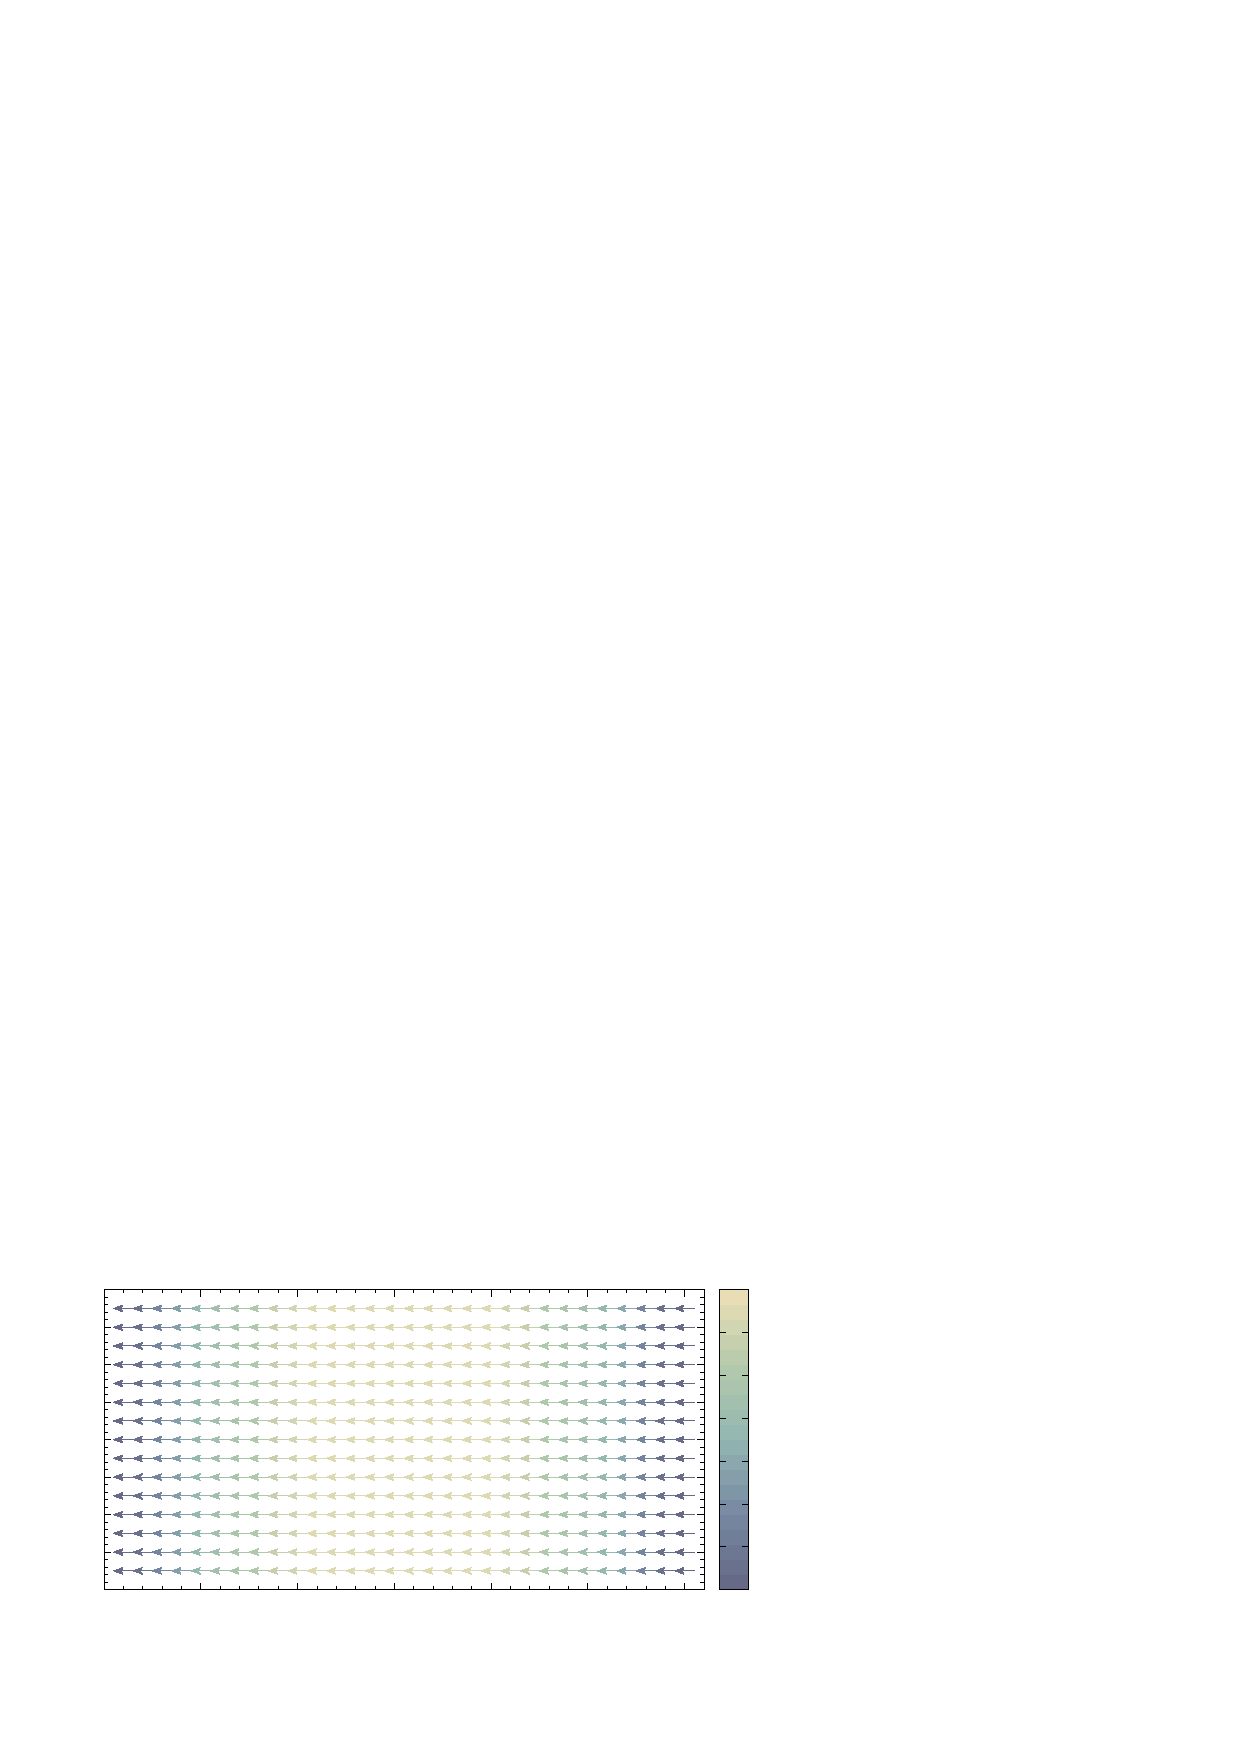
\includegraphics[width={288.00bp},height={188.60bp}]{Plots/SC10AM10/HeatMap/VertHorizBC/plot}}%
    \gplfronttext
  \end{picture}%
\endgroup


    \caption{Diagonal interface of a SC and an AM at $\mu = -1.5$.}
\end{figure}
\begin{figure}[H]
    \centering
    % GNUPLOT: LaTeX picture with Postscript
\begingroup
  % Encoding inside the plot.  In the header of your document, this encoding
  % should to defined, e.g., by using
  % \usepackage[cp1252,<other encodings>]{inputenc}
  \inputencoding{cp1252}%
  \makeatletter
  \providecommand\color[2][]{%
    \GenericError{(gnuplot) \space\space\space\@spaces}{%
      Package color not loaded in conjunction with
      terminal option `colourtext'%
    }{See the gnuplot documentation for explanation.%
    }{Either use 'blacktext' in gnuplot or load the package
      color.sty in LaTeX.}%
    \renewcommand\color[2][]{}%
  }%
  \providecommand\includegraphics[2][]{%
    \GenericError{(gnuplot) \space\space\space\@spaces}{%
      Package graphicx or graphics not loaded%
    }{See the gnuplot documentation for explanation.%
    }{The gnuplot epslatex terminal needs graphicx.sty or graphics.sty.}%
    \renewcommand\includegraphics[2][]{}%
  }%
  \providecommand\rotatebox[2]{#2}%
  \@ifundefined{ifGPcolor}{%
    \newif\ifGPcolor
    \GPcolortrue
  }{}%
  \@ifundefined{ifGPblacktext}{%
    \newif\ifGPblacktext
    \GPblacktextfalse
  }{}%
  % define a \g@addto@macro without @ in the name:
  \let\gplgaddtomacro\g@addto@macro
  % define empty templates for all commands taking text:
  \gdef\gplbacktext{}%
  \gdef\gplfronttext{}%
  \makeatother
  \ifGPblacktext
    % no textcolor at all
    \def\colorrgb#1{}%
    \def\colorgray#1{}%
  \else
    % gray or color?
    \ifGPcolor
      \def\colorrgb#1{\color[rgb]{#1}}%
      \def\colorgray#1{\color[gray]{#1}}%
      \expandafter\def\csname LTw\endcsname{\color{white}}%
      \expandafter\def\csname LTb\endcsname{\color{black}}%
      \expandafter\def\csname LTa\endcsname{\color{black}}%
      \expandafter\def\csname LT0\endcsname{\color[rgb]{1,0,0}}%
      \expandafter\def\csname LT1\endcsname{\color[rgb]{0,1,0}}%
      \expandafter\def\csname LT2\endcsname{\color[rgb]{0,0,1}}%
      \expandafter\def\csname LT3\endcsname{\color[rgb]{1,0,1}}%
      \expandafter\def\csname LT4\endcsname{\color[rgb]{0,1,1}}%
      \expandafter\def\csname LT5\endcsname{\color[rgb]{1,1,0}}%
      \expandafter\def\csname LT6\endcsname{\color[rgb]{0,0,0}}%
      \expandafter\def\csname LT7\endcsname{\color[rgb]{1,0.3,0}}%
      \expandafter\def\csname LT8\endcsname{\color[rgb]{0.5,0.5,0.5}}%
    \else
      % gray
      \def\colorrgb#1{\color{black}}%
      \def\colorgray#1{\color[gray]{#1}}%
      \expandafter\def\csname LTw\endcsname{\color{white}}%
      \expandafter\def\csname LTb\endcsname{\color{black}}%
      \expandafter\def\csname LTa\endcsname{\color{black}}%
      \expandafter\def\csname LT0\endcsname{\color{black}}%
      \expandafter\def\csname LT1\endcsname{\color{black}}%
      \expandafter\def\csname LT2\endcsname{\color{black}}%
      \expandafter\def\csname LT3\endcsname{\color{black}}%
      \expandafter\def\csname LT4\endcsname{\color{black}}%
      \expandafter\def\csname LT5\endcsname{\color{black}}%
      \expandafter\def\csname LT6\endcsname{\color{black}}%
      \expandafter\def\csname LT7\endcsname{\color{black}}%
      \expandafter\def\csname LT8\endcsname{\color{black}}%
    \fi
  \fi
    \setlength{\unitlength}{0.0500bp}%
    \ifx\gptboxheight\undefined%
      \newlength{\gptboxheight}%
      \newlength{\gptboxwidth}%
      \newsavebox{\gptboxtext}%
    \fi%
    \setlength{\fboxrule}{0.5pt}%
    \setlength{\fboxsep}{1pt}%
    \definecolor{tbcol}{rgb}{1,1,1}%
\begin{picture}(5760.00,3772.00)%
    \gplgaddtomacro\gplbacktext{%
      \csname LTb\endcsname%%
      \put(1807,3313){\makebox(0,0){\strut{}SC}}%
      \put(3953,3313){\makebox(0,0){\strut{}AM}}%
    }%
    \gplgaddtomacro\gplfronttext{%
      \csname LTb\endcsname%%
      \put(1073,742){\makebox(0,0){\scriptsize 2}}%
      \put(1525,742){\makebox(0,0){\scriptsize 4}}%
      \put(1977,742){\makebox(0,0){\scriptsize 6}}%
      \put(2429,742){\makebox(0,0){\scriptsize 8}}%
      \put(2880,742){\makebox(0,0){\scriptsize 10}}%
      \put(3331,742){\makebox(0,0){\scriptsize 12}}%
      \put(3783,742){\makebox(0,0){\scriptsize 14}}%
      \put(4235,742){\makebox(0,0){\scriptsize 16}}%
      \put(4687,742){\makebox(0,0){\scriptsize 18}}%
      \put(2880,478){\makebox(0,0){\small\textbf{Lattice site $i_x$ in $\bm{e}_x$}}}%
      \put(480,1006){\makebox(0,0){\scriptsize 2}}%
      \put(480,1254){\makebox(0,0){\scriptsize 4}}%
      \put(480,1501){\makebox(0,0){\scriptsize 6}}%
      \put(480,1749){\makebox(0,0){\scriptsize 8}}%
      \put(480,1996){\makebox(0,0){\scriptsize 10}}%
      \put(480,2243){\makebox(0,0){\scriptsize 12}}%
      \put(480,2491){\makebox(0,0){\scriptsize 14}}%
      \put(480,2738){\makebox(0,0){\scriptsize 16}}%
      \put(480,2986){\makebox(0,0){\scriptsize 18}}%
      \put(150,1996){\rotatebox{-270.00}{\makebox(0,0){\small\textbf{Lattice site $i_y$ in $\bm{e}_y$}}}}%
      \put(5743,820){\makebox(0,0){\tiny \(0\)}}%
      \put(5743,1212){\makebox(0,0){\tiny \(1e{-06}\)}}%
      \put(5743,1604){\makebox(0,0){\tiny \(2e{-06}\)}}%
      \put(5743,1996){\makebox(0,0){\tiny \(3e{-06}\)}}%
      \put(5743,2388){\makebox(0,0){\tiny \(4e{-06}\)}}%
      \put(5743,2780){\makebox(0,0){\tiny \(5e{-06}\)}}%
      \put(5743,3171){\makebox(0,0){\tiny \(6e{-06}\)}}%
    }%
    \gplbacktext
    \put(0,0){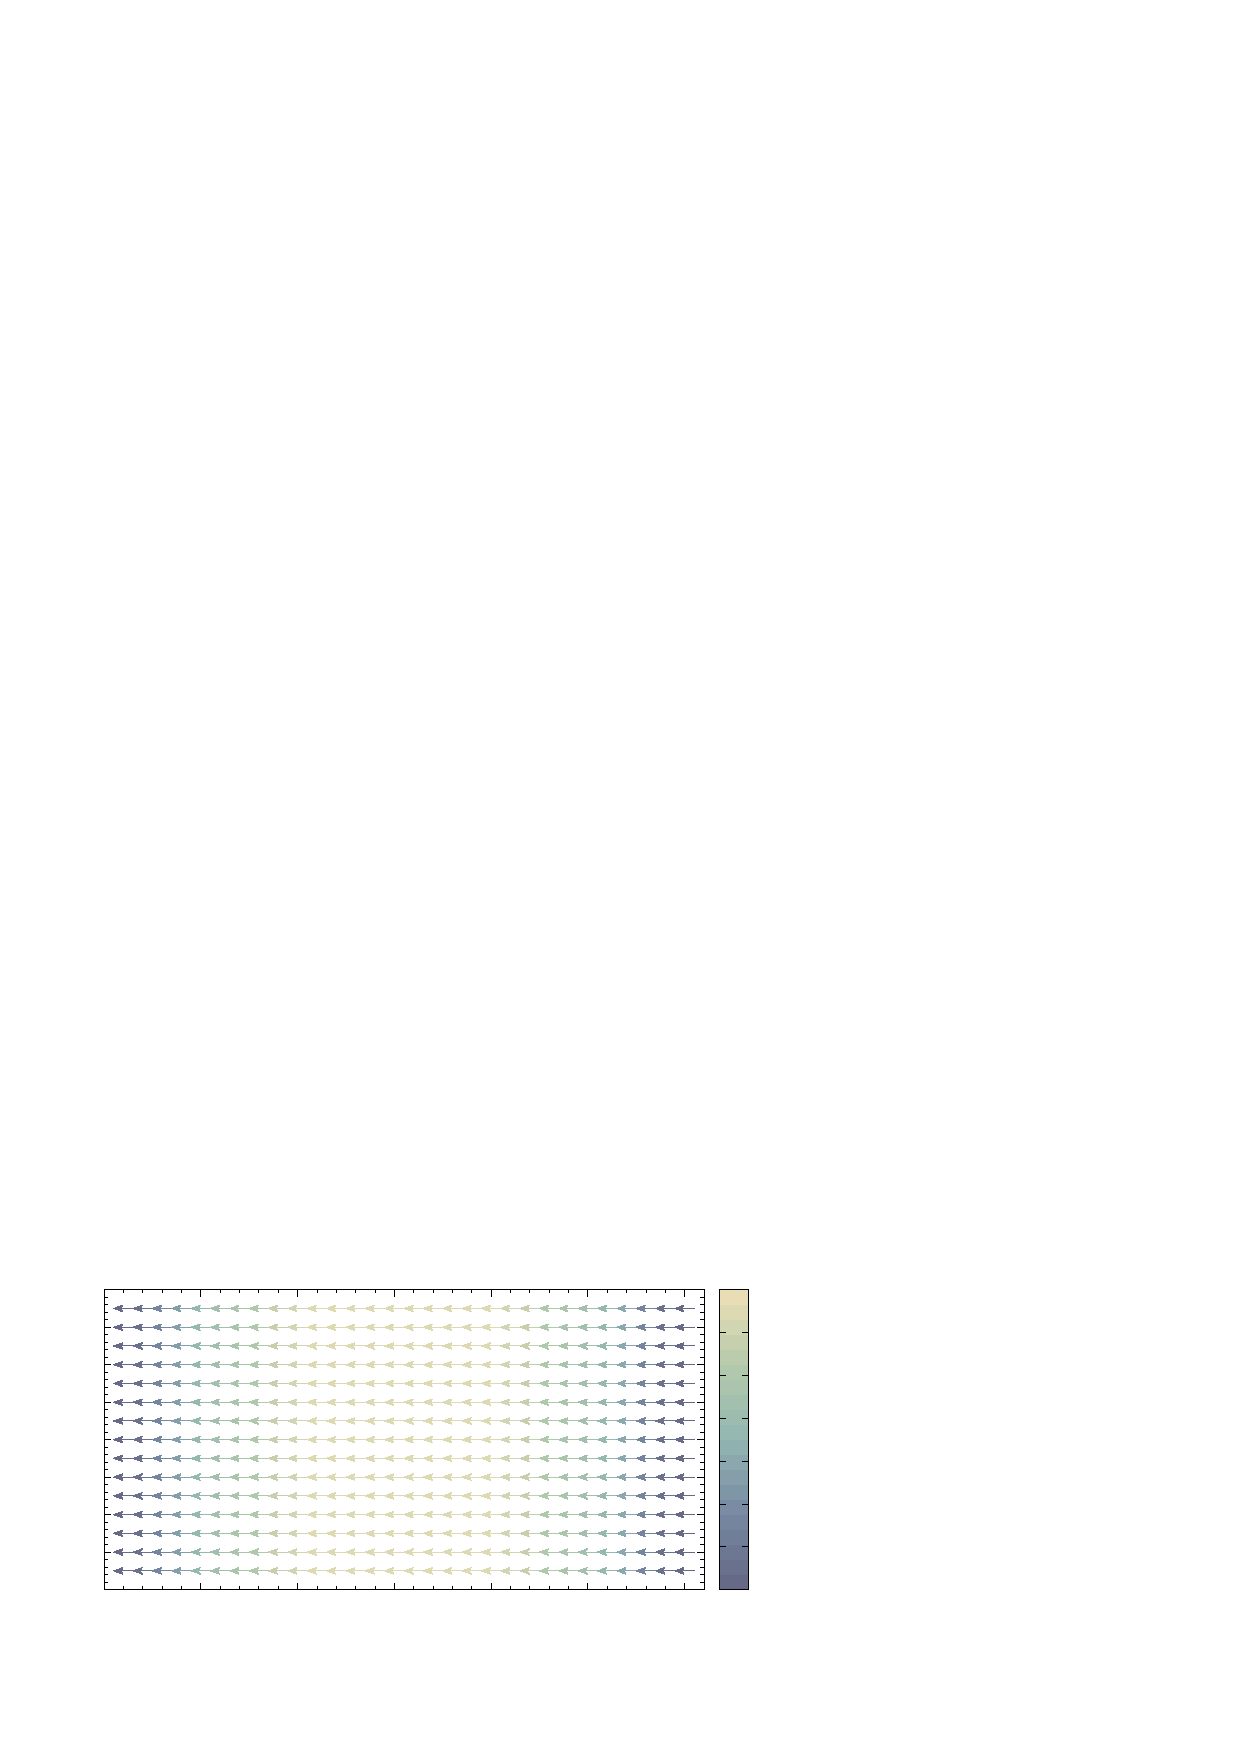
\includegraphics[width={288.00bp},height={188.60bp}]{Plots/SC10AM10/HeatMap/VertHorizBC/plot}}%
    \gplfronttext
  \end{picture}%
\endgroup


    \caption{Diagonal interface of a SC and an AM at $\mu = -0.5$.}
\end{figure}
The superconductivity fills uniformaly the superconductor. It's magnetude seams to grow while $|\mu|$ get closer to zero.
 

Once again the oscillating exponential decay is present. We count up to eight oscillations for the three cases of study, whose
frequency is arround three sites in all configurations. The oscillations takes only place along the $x$ axis but the exponential decay
seams to point along the normal of the interface, making the (40,0) region the less populated in Cooper pairs.
The lower the $|\mu|$, the less noise we observe in the plots. Similarly to the straight interface the decay is strong in the begging
and then slows down when approching the farest regions from the interface.\\

If we try to find the line for a given $y$ that has the same site length in the AM in the straight interface case, we can pick one the at $y=15$.
There we count the same number of oscillations in the AM than in the straight interface case. In fact at $y=1$ we can see that the AM was
extended and at $y=30$ we can see that the AM was shorten. This gives the room to more oscillations to happen in the first case,
and less in the second one. The profile of the oscilations \textit{along the $x$ axis} is the same than in the straight interface case. \\

In the same way than before, this increase in Cooper pairs formation with degrowing $|\mu|$ is due to the shape of the fermi surface.
Considering only the SC, we see an increase of an order of magnetude between $\mu=-2.5$ and $\mu=-1.5$. On the other hand we only count
a doubling of the Cooper pairs from $\mu=-1.5$ and $\mu=-0.5$.
As before the majority of the newly accessible states provided by $\mu=-0.5$ are outside the s-wave range.
This yields to a smaller increase in the number of Cooper pairs when compared to the first case.


We now that the Cooper pairs leak from the SC. We can reasonably say that they can leak in every direction from a site on the interface.
Due to interferences between them, we can expect to have a net diffusion along the normal of the interface. By doing so the leaking that we see
should be considered along the $(1,-1)$ axis: The leaking goes through the oscillations along the normal. This results in more spreaded
oscillations than in the straight interface case for the same traveled length.

\begin{figure}[H]
  \centering
  \includegraphics[width=0.5\textwidth]{Ressources/CooperPairsOrient.PNG}
  \caption{An arbitray oscillating exponential decay in the $x$-direction. Going this oscilations along $x$ or along the diagonal $(1,-1)$ axis results in different
  experienced oscilations for the same travel length. Plot made with Desmos.}
\end{figure}

\subsection{Conclusion and outlook}
We have seen that the BCS superconducting gap is influenced by the Fermi surface. The gap seams to be the biggest when the Fermi surface is the largest.
The gap is also influenced by the presence of impurities. We observe oscillations in the gap near the oben boundaries, whichare due to the reflection
of the quasiparticles with the sides.
Further we studied the leaking of the Cooper pairs in different materials. We observed an exponential decay in a normnal metal.
This decay is modulated by oscillations that are due to the spin-dependent hopping in both the ferro- and altermagnet.
Due to the axis-dependence of the hopping, the oscillations are stronger in the altermagnet than in the ferromagnet.\\
Adding a diagonal interface to the system, we observed the same exponential decay and oscillations. The oscillations are more spreaded when considering
the leaking of the Cooper pairs along the normal of the interface. This is due to the interference of the leaking Cooper pairs.\\
Towards the modelisation of a Josephon junction with an altermagnetic material, we achieved to represent the current in a superconductor.
The current seams to be proportional with the phase gradient of the superconducting gap and it's strength is grows with the number of Cooper pairs.
More work needs to be done to represent the current in the altermagnet between two diffent superconductors.\\

D-wave superconductivity was already introduced as being of particular interst. This is a more complex system:
The gap is now a neigbour dependent quantity and is not isotropic in the momentum space. Some work has been done towards studying the
proximity effect of a d-wave superconductor with the altermagnet. However by lack of time we only achieved to represent the d-wave in a superconductor.

\begin{figure}[H]
    % GNUPLOT: LaTeX picture with Postscript
\begingroup
  % Encoding inside the plot.  In the header of your document, this encoding
  % should to defined, e.g., by using
  % \usepackage[cp1252,<other encodings>]{inputenc}
  \inputencoding{cp1252}%
  \makeatletter
  \providecommand\color[2][]{%
    \GenericError{(gnuplot) \space\space\space\@spaces}{%
      Package color not loaded in conjunction with
      terminal option `colourtext'%
    }{See the gnuplot documentation for explanation.%
    }{Either use 'blacktext' in gnuplot or load the package
      color.sty in LaTeX.}%
    \renewcommand\color[2][]{}%
  }%
  \providecommand\includegraphics[2][]{%
    \GenericError{(gnuplot) \space\space\space\@spaces}{%
      Package graphicx or graphics not loaded%
    }{See the gnuplot documentation for explanation.%
    }{The gnuplot epslatex terminal needs graphicx.sty or graphics.sty.}%
    \renewcommand\includegraphics[2][]{}%
  }%
  \providecommand\rotatebox[2]{#2}%
  \@ifundefined{ifGPcolor}{%
    \newif\ifGPcolor
    \GPcolortrue
  }{}%
  \@ifundefined{ifGPblacktext}{%
    \newif\ifGPblacktext
    \GPblacktextfalse
  }{}%
  % define a \g@addto@macro without @ in the name:
  \let\gplgaddtomacro\g@addto@macro
  % define empty templates for all commands taking text:
  \gdef\gplbacktext{}%
  \gdef\gplfronttext{}%
  \makeatother
  \ifGPblacktext
    % no textcolor at all
    \def\colorrgb#1{}%
    \def\colorgray#1{}%
  \else
    % gray or color?
    \ifGPcolor
      \def\colorrgb#1{\color[rgb]{#1}}%
      \def\colorgray#1{\color[gray]{#1}}%
      \expandafter\def\csname LTw\endcsname{\color{white}}%
      \expandafter\def\csname LTb\endcsname{\color{black}}%
      \expandafter\def\csname LTa\endcsname{\color{black}}%
      \expandafter\def\csname LT0\endcsname{\color[rgb]{1,0,0}}%
      \expandafter\def\csname LT1\endcsname{\color[rgb]{0,1,0}}%
      \expandafter\def\csname LT2\endcsname{\color[rgb]{0,0,1}}%
      \expandafter\def\csname LT3\endcsname{\color[rgb]{1,0,1}}%
      \expandafter\def\csname LT4\endcsname{\color[rgb]{0,1,1}}%
      \expandafter\def\csname LT5\endcsname{\color[rgb]{1,1,0}}%
      \expandafter\def\csname LT6\endcsname{\color[rgb]{0,0,0}}%
      \expandafter\def\csname LT7\endcsname{\color[rgb]{1,0.3,0}}%
      \expandafter\def\csname LT8\endcsname{\color[rgb]{0.5,0.5,0.5}}%
    \else
      % gray
      \def\colorrgb#1{\color{black}}%
      \def\colorgray#1{\color[gray]{#1}}%
      \expandafter\def\csname LTw\endcsname{\color{white}}%
      \expandafter\def\csname LTb\endcsname{\color{black}}%
      \expandafter\def\csname LTa\endcsname{\color{black}}%
      \expandafter\def\csname LT0\endcsname{\color{black}}%
      \expandafter\def\csname LT1\endcsname{\color{black}}%
      \expandafter\def\csname LT2\endcsname{\color{black}}%
      \expandafter\def\csname LT3\endcsname{\color{black}}%
      \expandafter\def\csname LT4\endcsname{\color{black}}%
      \expandafter\def\csname LT5\endcsname{\color{black}}%
      \expandafter\def\csname LT6\endcsname{\color{black}}%
      \expandafter\def\csname LT7\endcsname{\color{black}}%
      \expandafter\def\csname LT8\endcsname{\color{black}}%
    \fi
  \fi
    \setlength{\unitlength}{0.0500bp}%
    \ifx\gptboxheight\undefined%
      \newlength{\gptboxheight}%
      \newlength{\gptboxwidth}%
      \newsavebox{\gptboxtext}%
    \fi%
    \setlength{\fboxrule}{0.5pt}%
    \setlength{\fboxsep}{1pt}%
    \definecolor{tbcol}{rgb}{1,1,1}%
\begin{picture}(8640.00,3772.00)%
    \gplgaddtomacro\gplbacktext{%
      \csname LTb\endcsname%%
      \put(1122,1728){\makebox(0,0){\scriptsize 1e-06}}%
      \put(1122,2063){\makebox(0,0){\scriptsize 1e-05}}%
      \put(1122,2399){\makebox(0,0){\scriptsize 0.0001}}%
      \put(1122,2734){\makebox(0,0){\scriptsize 0.001}}%
      \put(1122,3069){\makebox(0,0){\scriptsize 0.01}}%
      \put(1122,3405){\makebox(0,0){\scriptsize 0.1}}%
      \put(1122,3740){\makebox(0,0){\scriptsize 1}}%
      \put(2092,1596){\makebox(0,0){\strut{}}}%
      \put(2975,1596){\makebox(0,0){\strut{}}}%
      \put(3858,1596){\makebox(0,0){\strut{}}}%
      \put(4741,1596){\makebox(0,0){\strut{}}}%
      \put(5624,1596){\makebox(0,0){\strut{}}}%
      \put(6507,1596){\makebox(0,0){\strut{}}}%
      \put(3947,3861){\makebox(0,0){\strut{}SC}}%
    }%
    \gplgaddtomacro\gplfronttext{%
      \csname LTb\endcsname%%
      \put(7626,2498){\makebox(0,0)[l]{\strut{}\footnotesize -3.75}}%
      \csname LTb\endcsname%%
      \put(7626,2278){\makebox(0,0)[l]{\strut{}\footnotesize -2.75}}%
      \csname LTb\endcsname%%
      \put(7626,2058){\makebox(0,0)[l]{\strut{}\footnotesize -1.75}}%
      \csname LTb\endcsname%%
      \put(7626,1838){\makebox(0,0)[l]{\strut{}\footnotesize -0.75}}%
      \csname LTb\endcsname%%
      \put(7626,1618){\makebox(0,0)[l]{\strut{}\footnotesize 0.75}}%
      \csname LTb\endcsname%%
      \put(7626,1398){\makebox(0,0)[l]{\strut{}\footnotesize 1.75}}%
      \csname LTb\endcsname%%
      \put(7626,1178){\makebox(0,0)[l]{\strut{}\footnotesize 2.75}}%
      \csname LTb\endcsname%%
      \put(7626,958){\makebox(0,0)[l]{\strut{}\footnotesize 3.75}}%
      \csname LTb\endcsname%%
      \put(253,2074){\rotatebox{-270.00}{\makebox(0,0){\strut{}$\bm{|F_d|}$}}}%
    }%
    \gplgaddtomacro\gplbacktext{%
      \csname LTb\endcsname%%
      \put(1115,843){\makebox(0,0){\scriptsize 1e-13}}%
      \put(1115,1383){\makebox(0,0){\scriptsize 1e-12}}%
      \put(2087,711){\makebox(0,0){ \(5\)}}%
      \put(2971,711){\makebox(0,0){ \(10\)}}%
      \put(3856,711){\makebox(0,0){ \(15\)}}%
      \put(4741,711){\makebox(0,0){ \(20\)}}%
      \put(5625,711){\makebox(0,0){ \(25\)}}%
      \put(6510,711){\makebox(0,0){ \(30\)}}%
    }%
    \gplgaddtomacro\gplfronttext{%
      \csname LTb\endcsname%%
      \put(3944,436){\makebox(0,0){\small\textbf{Lattice site $i$ in $\bm{e}_x$}}}%
    }%
    \gplbacktext
    \put(0,0){\includegraphics[width={432.00bp},height={188.60bp}]{../Plots/SC30/DWave/StraightInterface/FreeDelta/diffMUplot}}%
    \gplfronttext
  \end{picture}%
\endgroup


    \caption{D wave with free delta and real $\Delta_d$}
\end{figure}


% \begin{tikzpicture}
%     \begin{axis}[
%         view={0}{90},  % Adjust the viewing angle
%         axis lines=center,
%         xlabel={$x$}, ylabel={$y$}, zlabel={$z$},
%         domain=-2*pi:2*pi, domain y=-2*pi:2*pi,
%         colormap/cool,
%       ]
%       % \addplot3[
%       %   surf,
%       %   shader=flat,
%       %   samples=50,
%       %   samples y=50,
%       %   z buffer=sort,
%       %   unbounded coords=jump,
%       % ]
%       % ({fd(x)},{y},{fd(x)}); % Using fd(x) for z-value

%       \addplot3[
%         surf,
%         shader=flat,
%         samples=100,
%         samples y=100,
%         z buffer=sort,
%         unbounded coords=jump,
%       ]
%       ({x},{y},{f(x,y,2)}); % Change th{f(x,y,0.5)}e last parameter (2) to set "a" \pgfmathifthenelse{abs(cos(x-pi) + cos(y-pi) - 2/2) < 1e-3}{2}{-2}}
%     \end{axis}
%   \end{tikzpicture}
\rem{A side view to comapre the oscilation amplitude.}


\end{document}